\section{System Architectural Models (Modelli OOA)}

La presente sezione descrive l'architettura dinamica e strutturale del sistema \textbf{MyAma} mediante i modelli di \textit{Object Oriented Analysis} (OOA) sviluppati con il tool Visual Paradigm.

% =========================================================================
% 5.1 ACTIVITY DIAGRAMS
% =========================================================================
\subsection{Activity Diagrams}
Gli Activity Diagram descrivono i flussi operativi, le diramazioni decisionali e i punti di sincronizzazione nei processi cardine della piattaforma. Di seguito vengono presentati i diagrammi fondamentali, raggruppati per attore, al fine di modellare compiutamente la dinamica dell'intero sistema MyAma.

\subsubsection{Utente non registrato e Utente di sistema}
Questi diagrammi modellano i flussi di base per l'ingresso nel sistema, dalla registrazione fino all'autenticazione.

\begin{figure}[H]
    \centering
    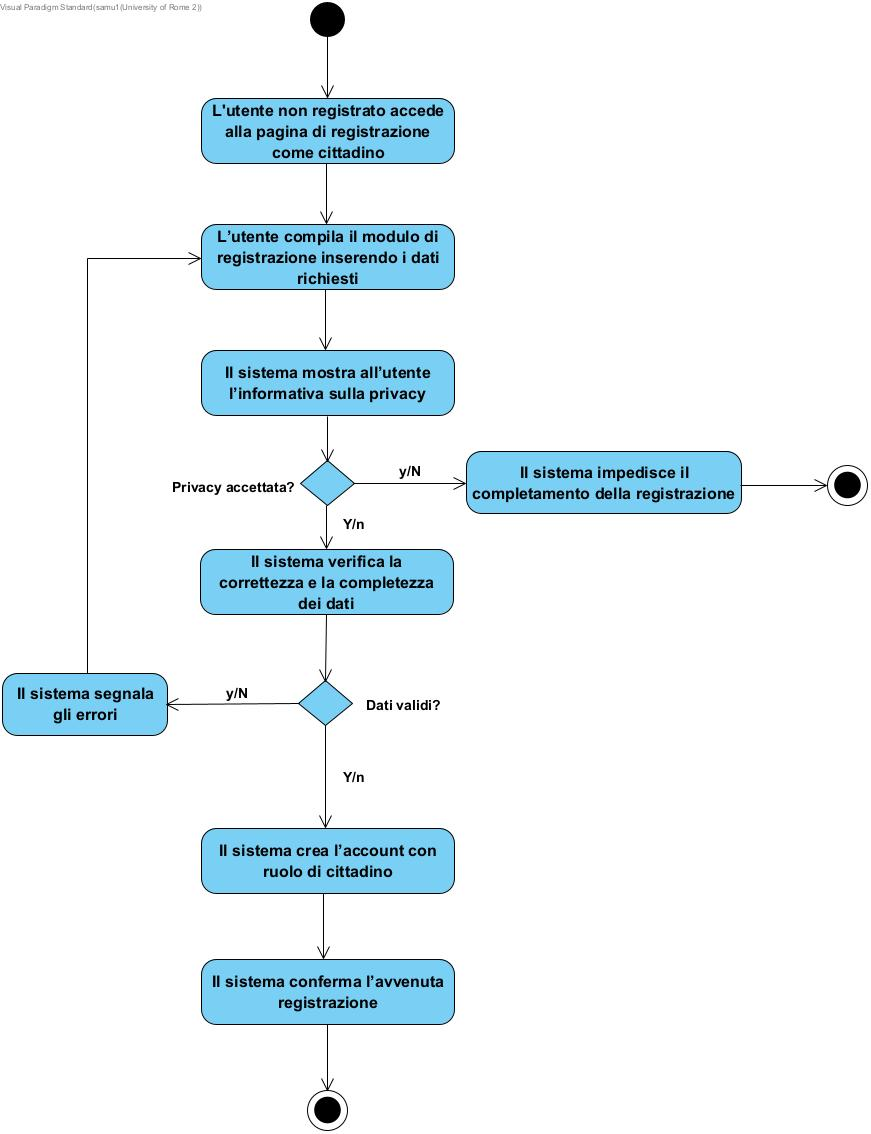
\includegraphics[width=\textwidth,height=0.70\textheight,keepaspectratio]{figure/act_registrarsi_cittadino.jpg}
    \caption{Activity Diagram --- Registrarsi come cittadino}
\end{figure}

\begin{figure}[H]
    \centering
    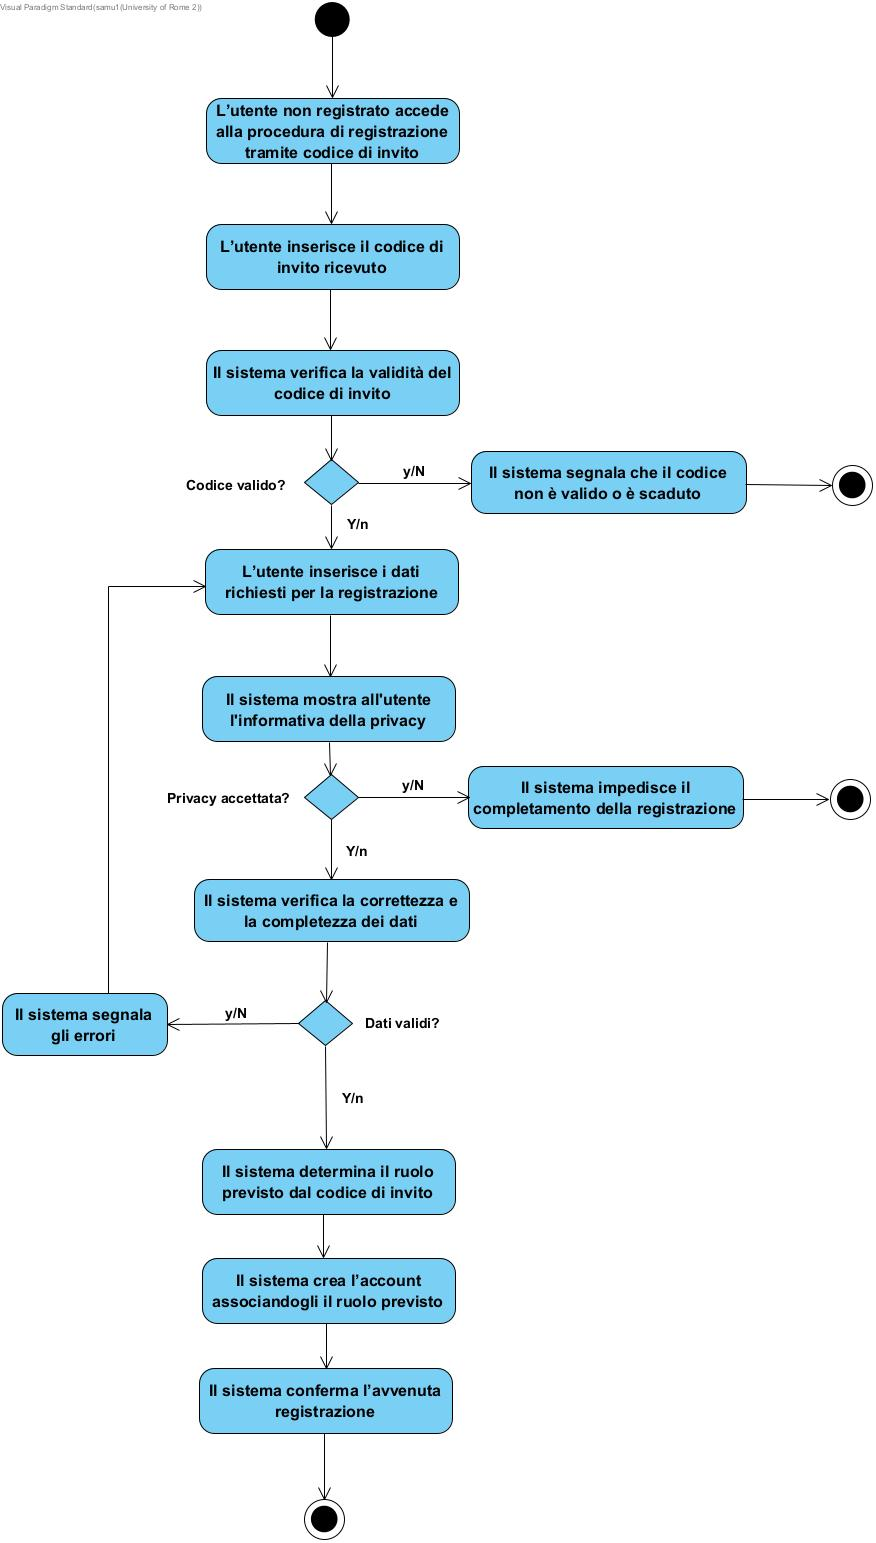
\includegraphics[width=\textwidth,height=0.70\textheight,keepaspectratio]{figure/act_registrarsi_invito.jpg}
    \caption{Activity Diagram --- Registrarsi tramite codice di invito}
\end{figure}

\begin{figure}[H]
    \centering
    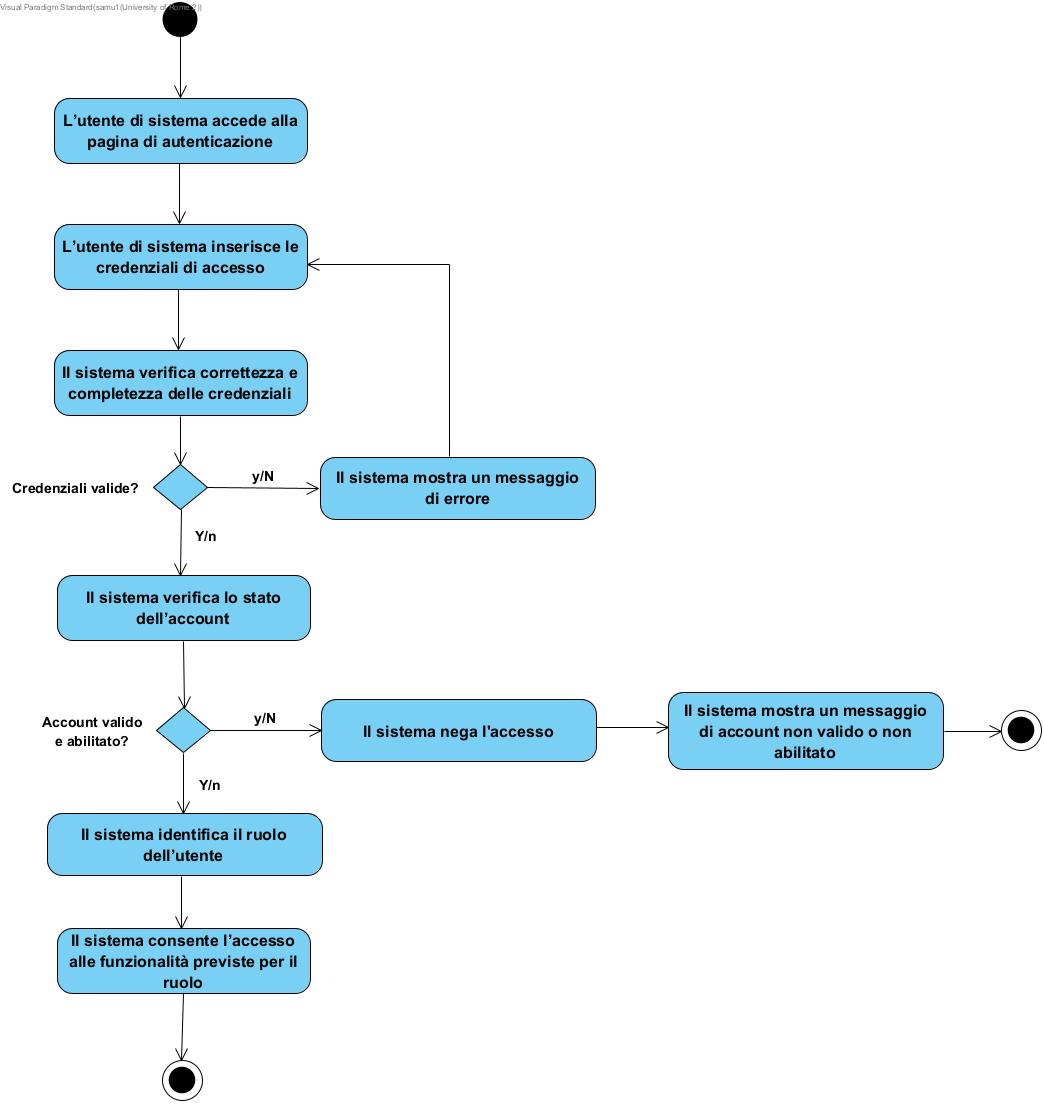
\includegraphics[width=\textwidth,height=0.70\textheight,keepaspectratio]{figure/act_effettuare_accesso.jpg}
    \caption{Activity Diagram --- Effettuare accesso}
\end{figure}

\subsubsection{Cittadino}
I seguenti diagrammi illustrano le interazioni del cittadino per usufruire dei servizi AMA, dalla prenotazione fino alla valutazione finale.

\begin{figure}[H]
    \centering
    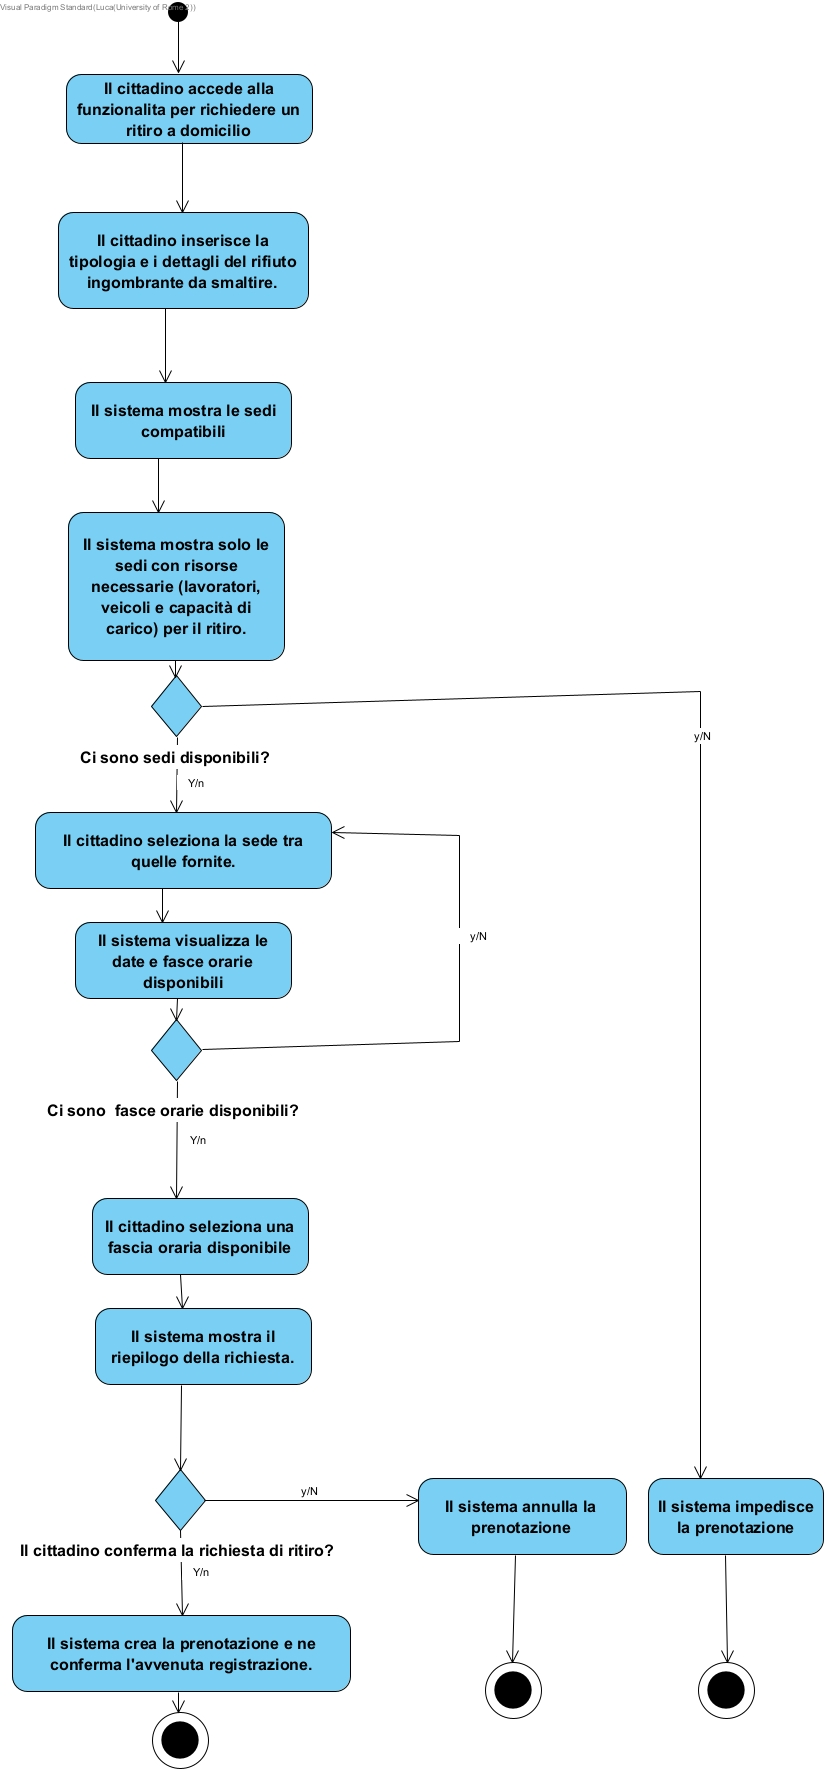
\includegraphics[width=\textwidth,height=0.70\textheight,keepaspectratio]{figure/act_richiesta_ritiro.jpg}
    \caption{Activity Diagram --- Richiesta ritiro a domicilio}
\end{figure}

\begin{figure}[H]
    \centering
    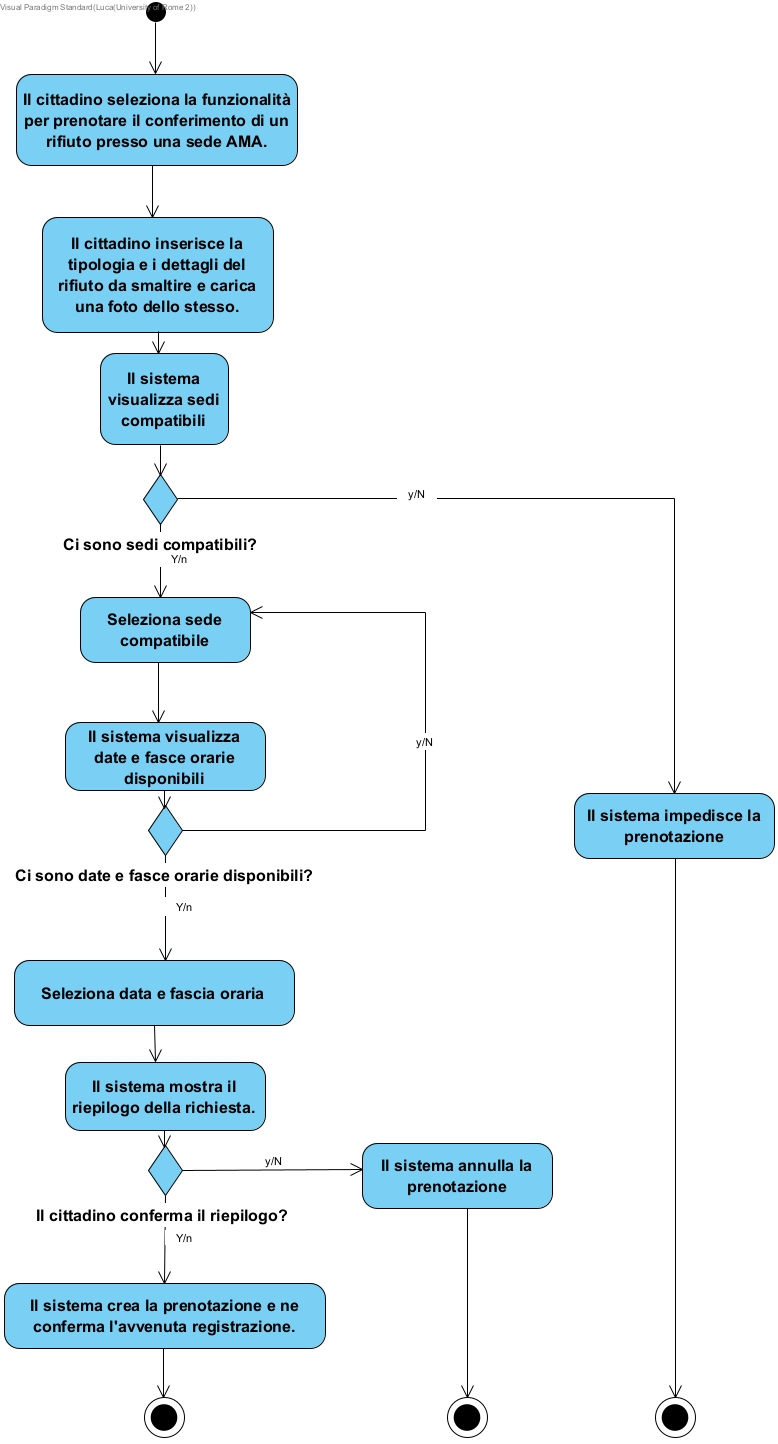
\includegraphics[width=\textwidth,height=0.70\textheight,keepaspectratio]{figure/act_prenota_conferimento.jpg}
    \caption{Activity Diagram --- Prenotare conferimento in sede}
\end{figure}

\begin{figure}[H]
    \centering
    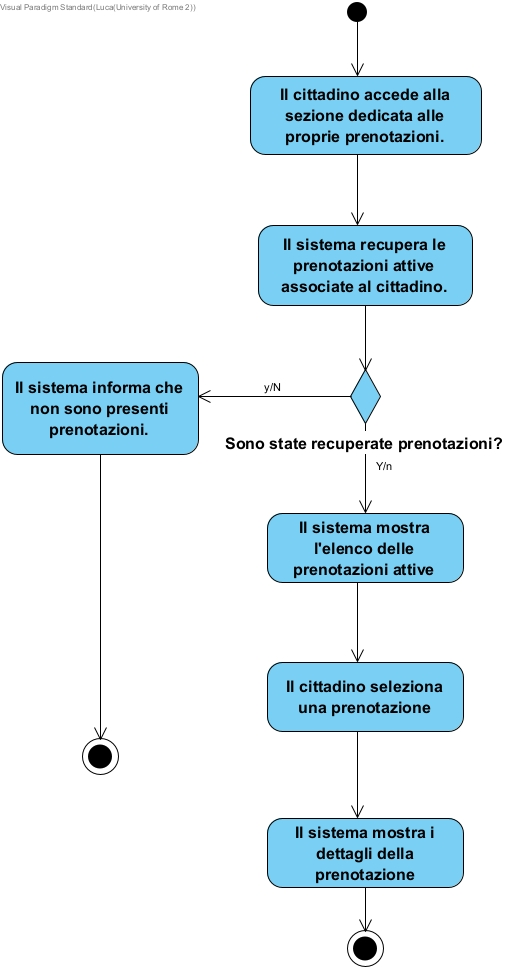
\includegraphics[width=\textwidth,height=0.70\textheight,keepaspectratio]{figure/act_visualizzare_prenotazioni.jpg}
    \caption{Activity Diagram --- Visualizzare prenotazioni attive}
\end{figure}

\begin{figure}[H]
    \centering
    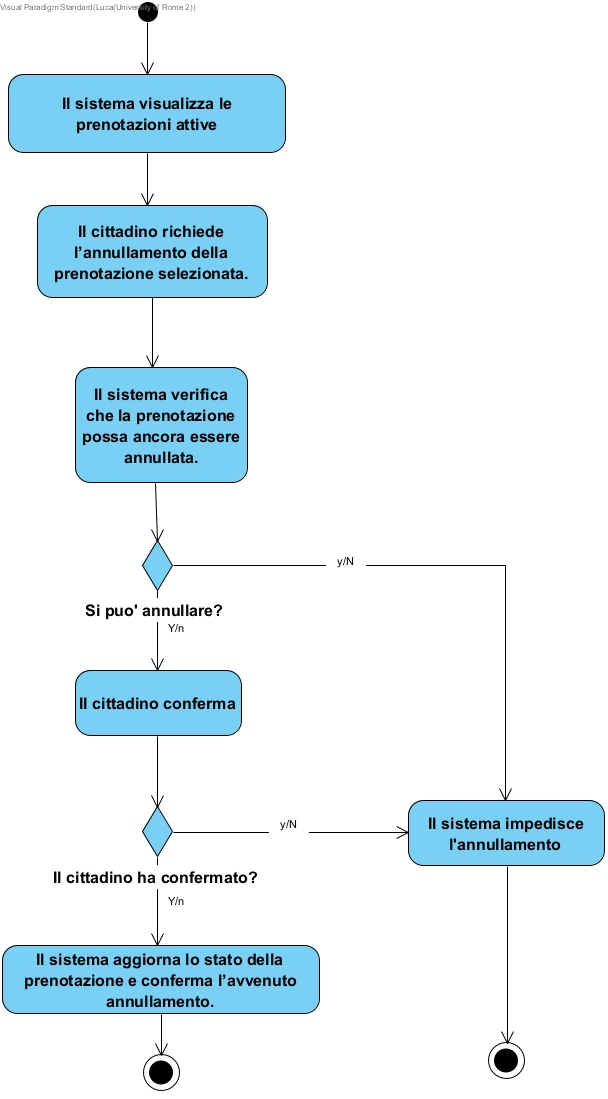
\includegraphics[width=\textwidth,height=0.70\textheight,keepaspectratio]{figure/act_annullare_prenotazione.jpg}
    \caption{Activity Diagram --- Annullare prenotazione}
\end{figure}

\begin{figure}[H]
    \centering
    
\includegraphics[width=\textwidth,height=0.70\textheight,keepaspectratio]{figure/act_valutare_servizio.jpg}
    \caption{Activity Diagram --- Valutare il servizio}
\end{figure}

\subsubsection{Autista e Operatore di Sede AMA}
Questi diagrammi modellano il flusso di lavoro logistico del personale sul campo: lo svolgimento del servizio, i controlli di conformità e la registrazione dell'esito.

\begin{figure}[H]
    \centering
    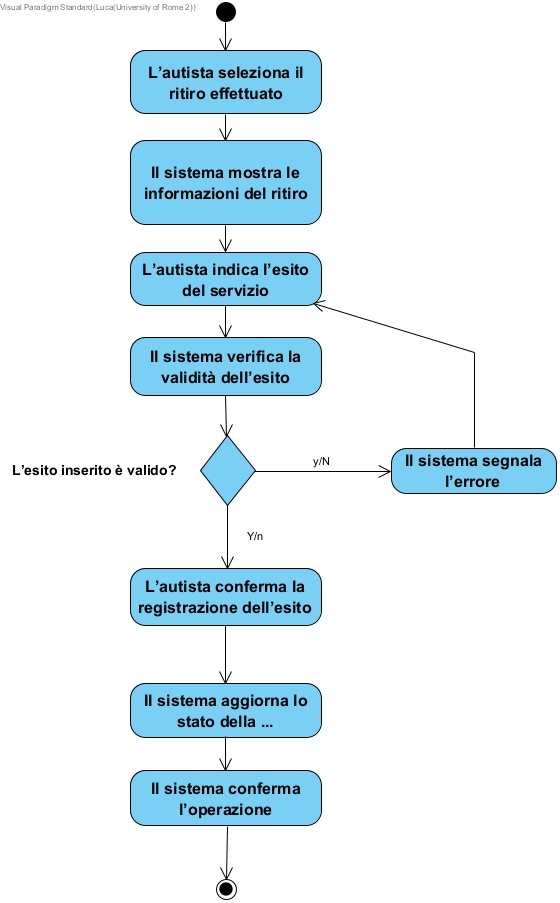
\includegraphics[width=\textwidth,height=0.70\textheight,keepaspectratio]{figure/act_autista_registrare_esito.jpg}
    \caption{Activity Diagram --- Registrare esito del ritiro (Autista)}
\end{figure}

\begin{figure}[H]
    \centering
    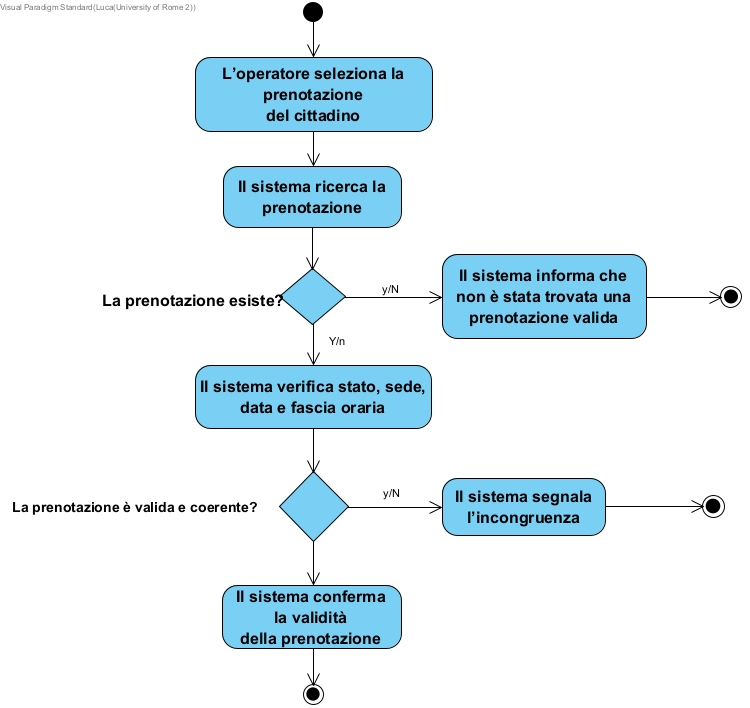
\includegraphics[width=\textwidth,height=0.70\textheight,keepaspectratio]{figure/act_operatore_verificare.jpg}
    \caption{Activity Diagram --- Verificare prenotazione del cittadino (Operatore di Sede)}
\end{figure}

\begin{figure}[H]
    \centering
    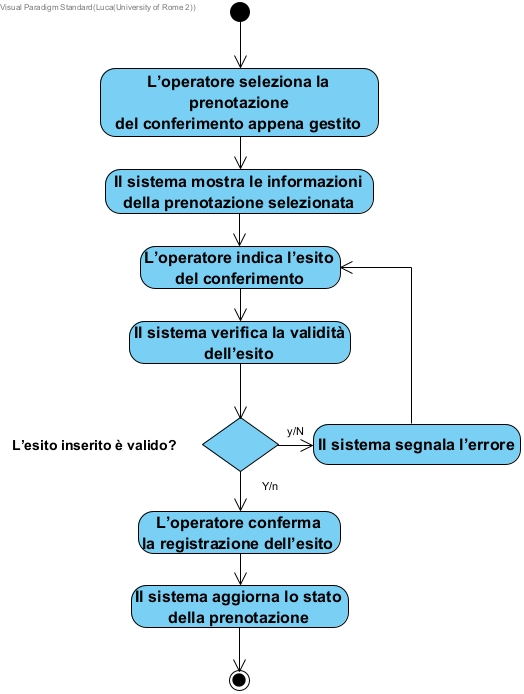
\includegraphics[width=\textwidth,height=0.70\textheight,keepaspectratio]{figure/act_operatore_esito_conferimento.jpg}
    \caption{Activity Diagram --- Registrare esito del conferimento (Operatore di Sede)}
\end{figure}

\subsubsection{Amministratori (di Sede e Generale)}
I processi amministrativi consentono di gestire le risorse umane, i mezzi logistici e la configurazione strutturale delle sedi.

\begin{figure}[H]
    \centering
    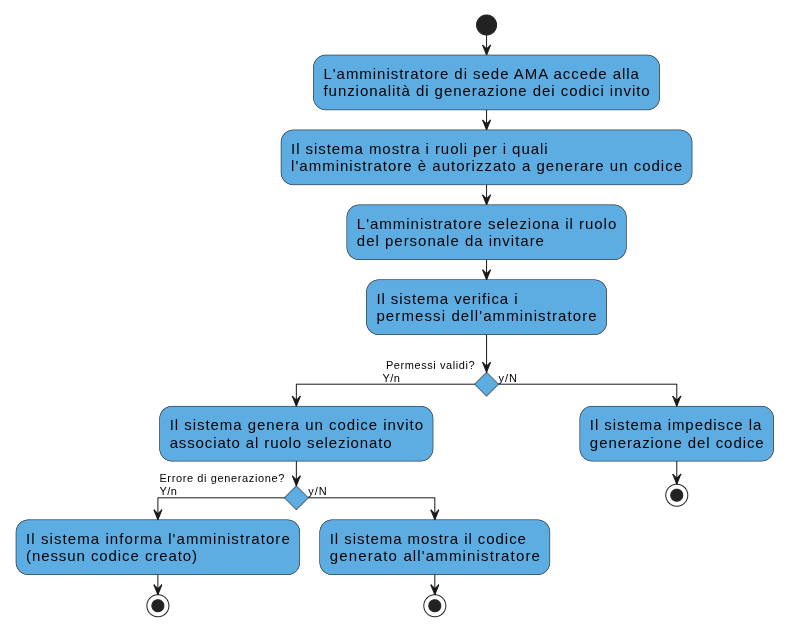
\includegraphics[width=\textwidth,height=0.70\textheight,keepaspectratio]{figure/act_admin_sede_genera_codice.png}
    \caption{Activity Diagram --- Generare codice di invito (Amministratore Sede)}
\end{figure}

\begin{figure}[H]
    \centering
    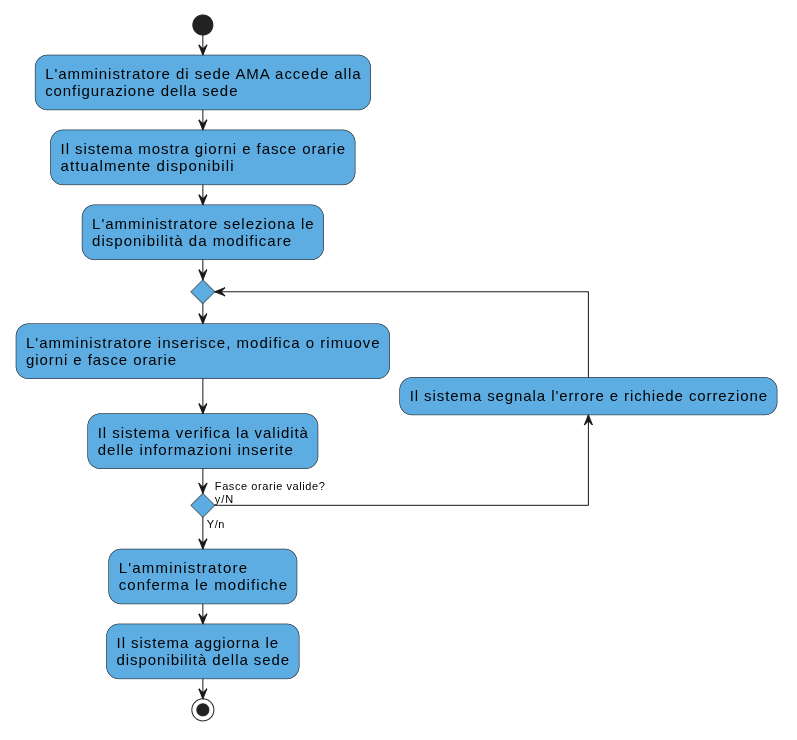
\includegraphics[width=\textwidth,height=0.70\textheight,keepaspectratio]{figure/act_admin_sede_gestire_fasce.png}
    \caption{Activity Diagram --- Gestire disponibilità della sede e fasce orarie}
\end{figure}

\begin{figure}[H]
    \centering
    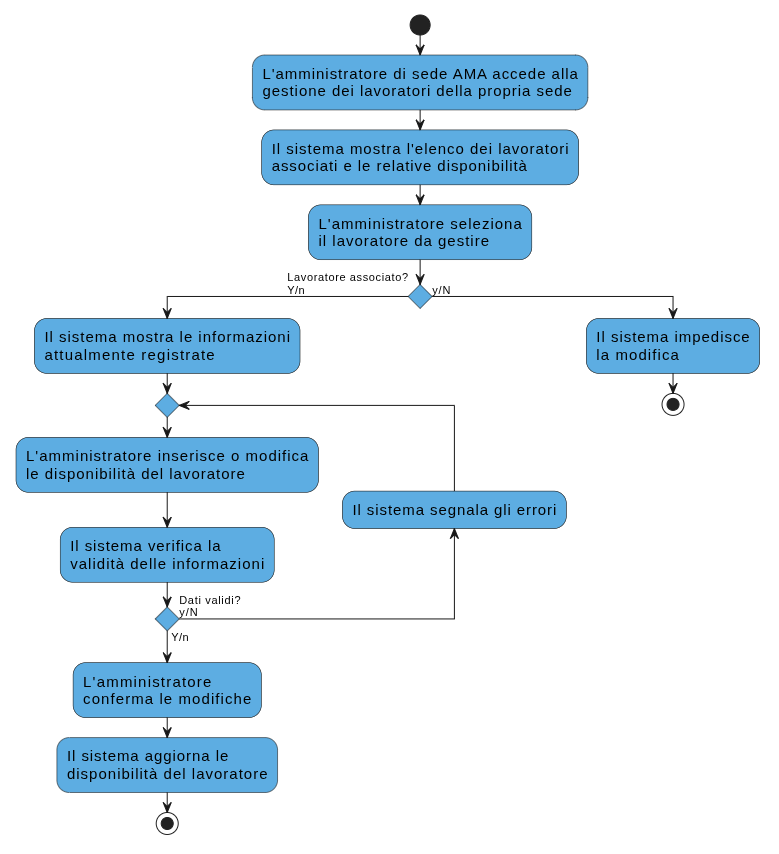
\includegraphics[width=\textwidth,height=0.70\textheight,keepaspectratio]{figure/act_admin_sede_gestire_lavoratori.png}
    \caption{Activity Diagram --- Gestire disponibilità dei lavoratori}
\end{figure}

\begin{figure}[H]
    \centering
    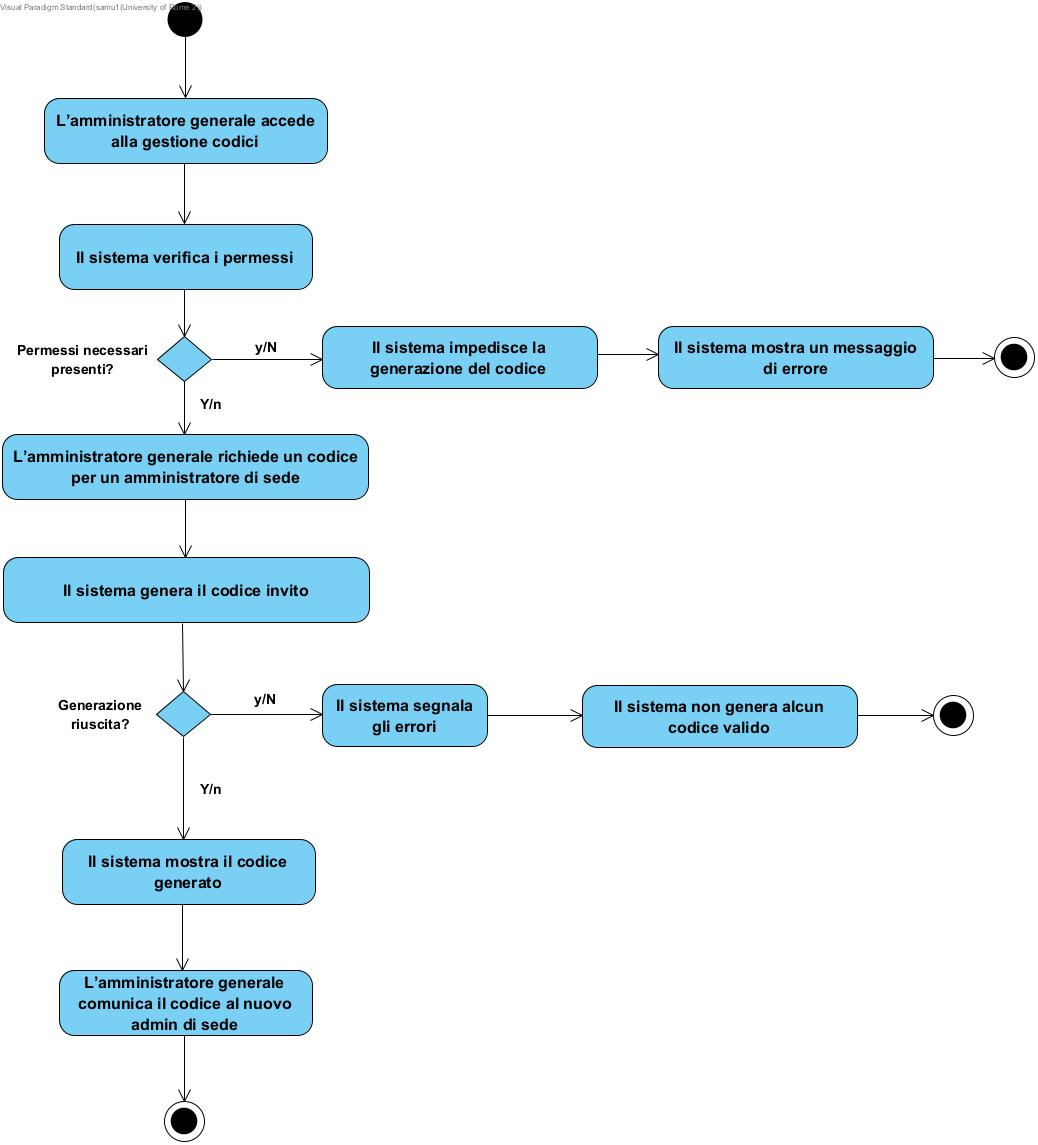
\includegraphics[width=\textwidth,height=0.70\textheight,keepaspectratio]{figure/act_generare_codice_admin.jpg}
    \caption{Activity Diagram --- Generare codice amministratore di sede (Amministratore Generale)}
\end{figure}

% =========================================================================
% 5.2 SEQUENCE DIAGRAMS
% =========================================================================
\subsection{Sequence Diagrams}
I Sequence Diagram descrivono l'interazione temporale tra gli oggetti del sistema durante l'esecuzione dei casi d'uso, applicando il pattern architetturale \textbf{BCE} (\textit{Boundary}, \textit{Control}, \textit{Entity}). Di seguito sono riportati i diagrammi principali, raggruppati per attore.

\subsubsection{Utente non registrato e Utente di sistema}

\begin{figure}[H]
    \centering
    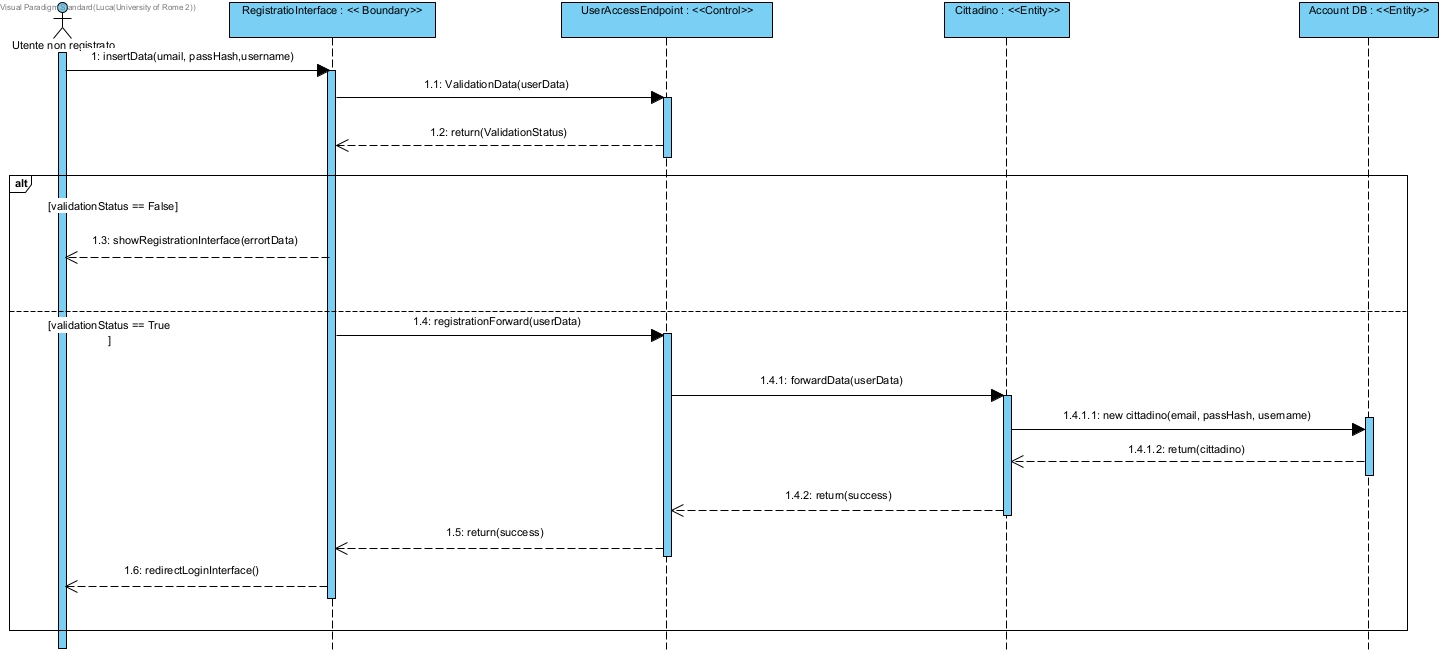
\includegraphics[width=\textwidth,height=0.70\textheight,keepaspectratio]{figure/seq_Utente_non_Registrazione_cittadino.jpg}
    \caption{Sequence Diagram --- Registrarsi come cittadino}
\end{figure}

\begin{figure}[H]
    \centering
    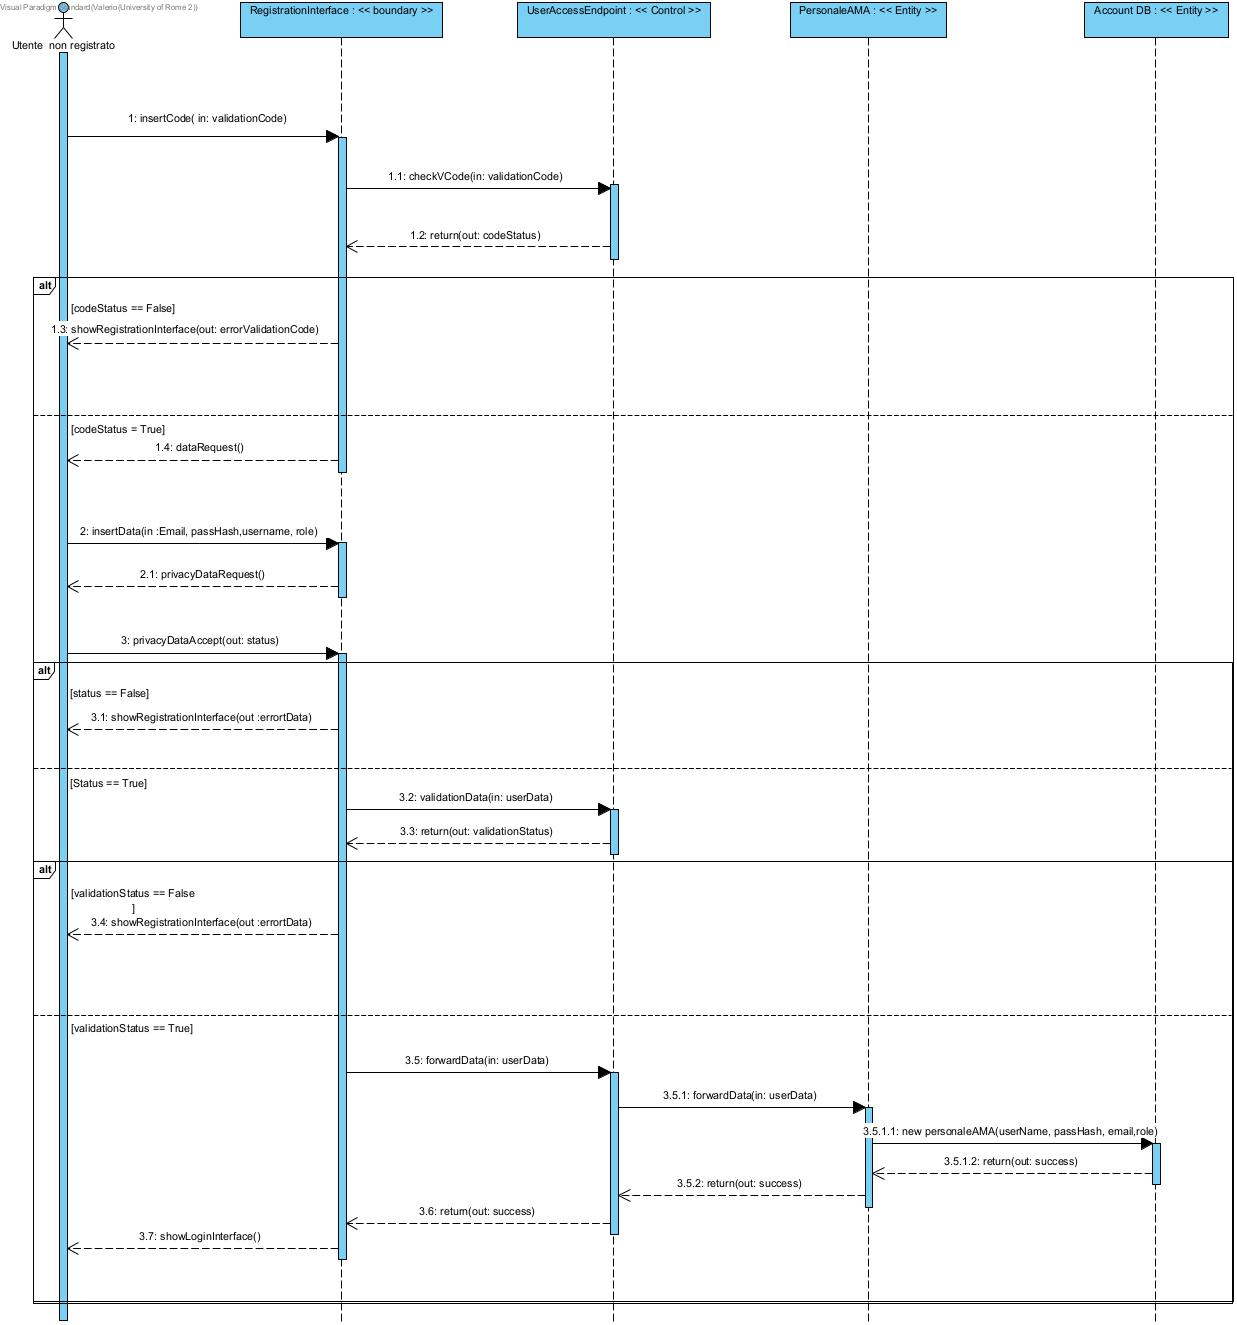
\includegraphics[width=\textwidth,height=0.70\textheight,keepaspectratio]{figure/seq_registrazione_Tramite_codice_invito.jpg}
    \caption{Sequence Diagram --- Registrarsi tramite codice di invito}
\end{figure}

\begin{figure}[H]
    \centering
    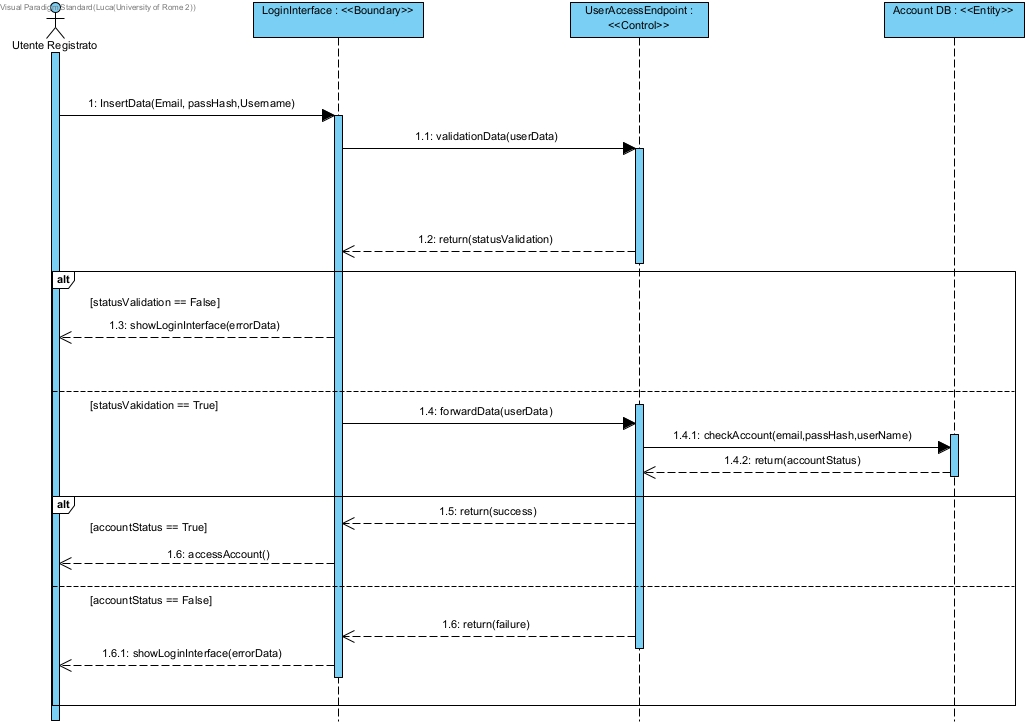
\includegraphics[width=\textwidth,height=0.70\textheight,keepaspectratio]{figure/seq_EseguiAccesso.jpg}
    \caption{Sequence Diagram --- Effettuare accesso}
\end{figure}

\subsubsection{Cittadino}

\begin{figure}[H]
    \centering
    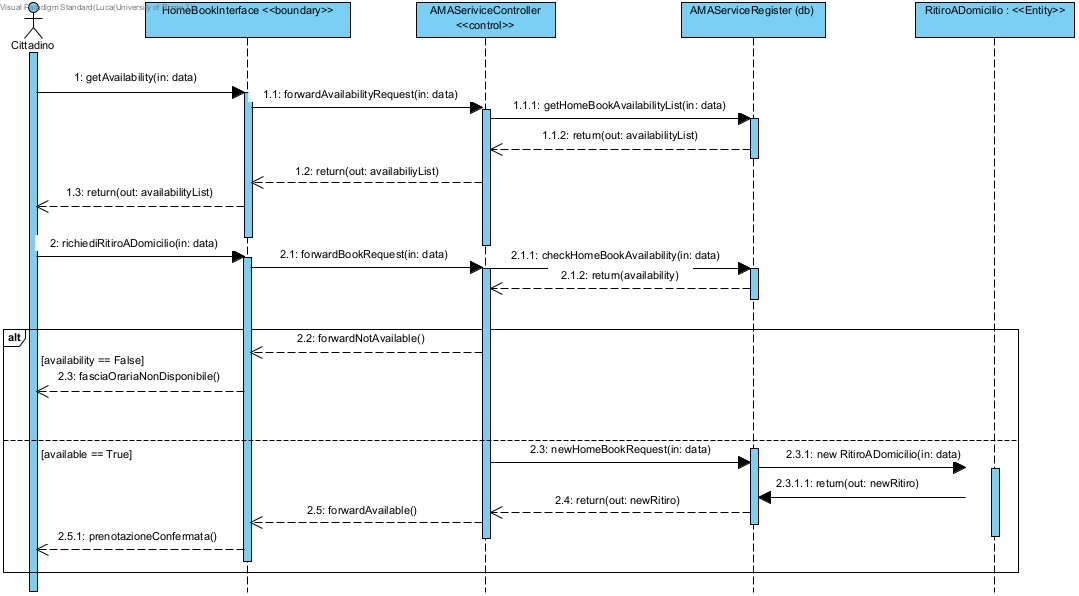
\includegraphics[width=\textwidth,height=0.70\textheight,keepaspectratio]{figure/seq_DiagramRichiedereRitiroADomicilio.jpg}
    \caption{Sequence Diagram --- Richiedere ritiro a domicilio}
\end{figure}

\begin{figure}[H]
    \centering
    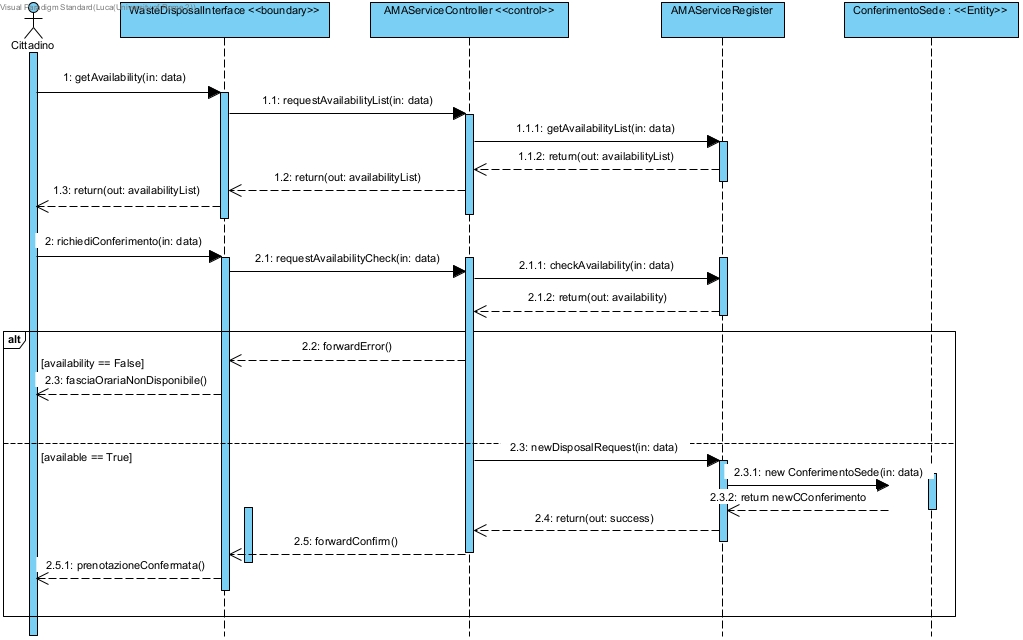
\includegraphics[width=\textwidth,height=0.70\textheight,keepaspectratio]{figure/seq_DiagramPrenotaConferimento.jpg}
    \caption{Sequence Diagram --- Prenotare conferimento presso sede AMA}
\end{figure}

\begin{figure}[H]
    \centering
    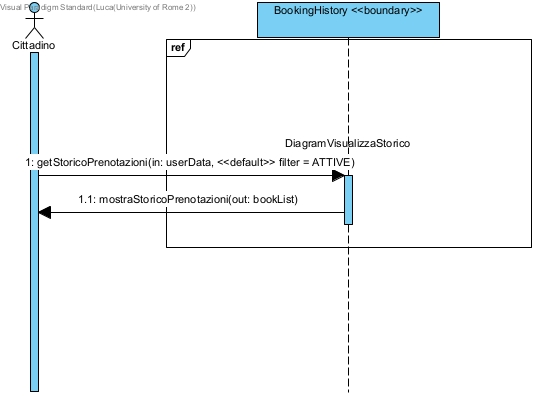
\includegraphics[width=\textwidth,height=0.70\textheight,keepaspectratio]{figure/seq_DiagramVisualizzarePrenotazioniAttive.jpg}
    \caption{Sequence Diagram --- Visualizzare prenotazioni attive}
\end{figure}

\begin{figure}[H]
    \centering
    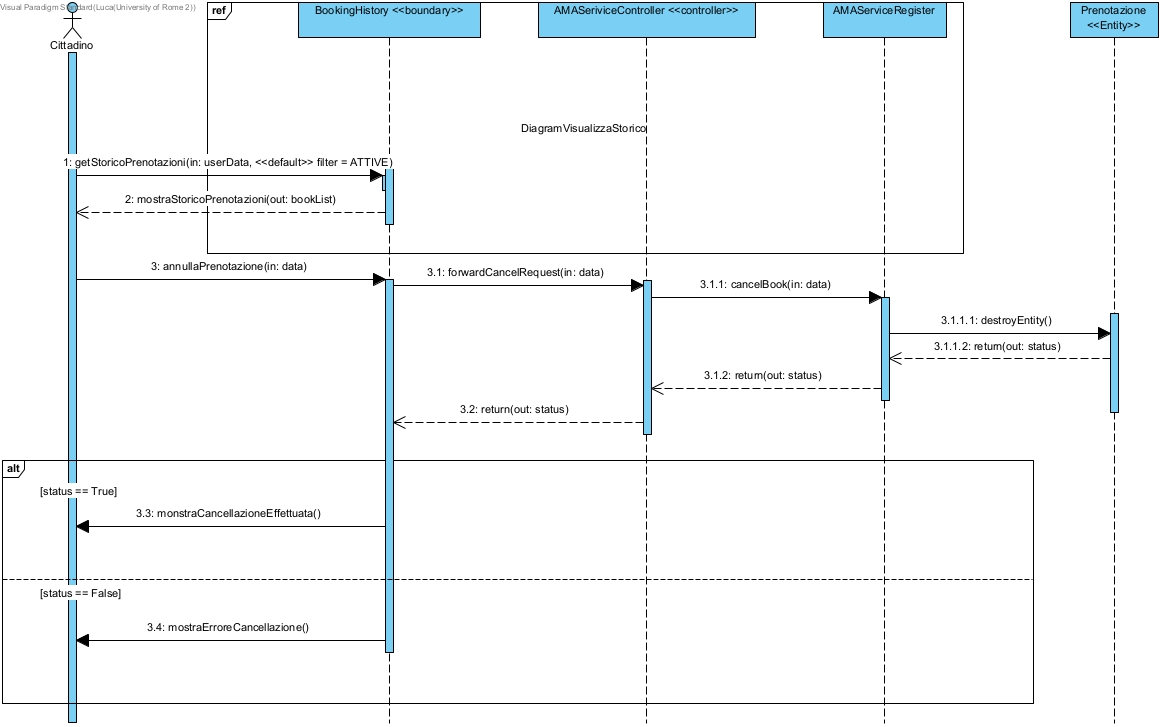
\includegraphics[width=\textwidth,height=0.70\textheight,keepaspectratio]{figure/seq_DiagramAnnullarePrenotazione.jpg}
    \caption{Sequence Diagram --- Annullare prenotazione}
\end{figure}

\begin{figure}[H]
    \centering
    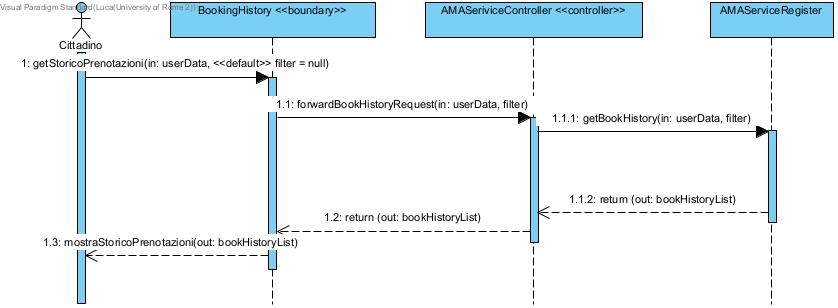
\includegraphics[width=\textwidth,height=0.70\textheight,keepaspectratio]{figure/seq_DiagramVisualizzaStorico.jpg}
    \caption{Sequence Diagram --- Visualizzare storico prenotazioni}
\end{figure}

\begin{figure}[H]
    \centering
    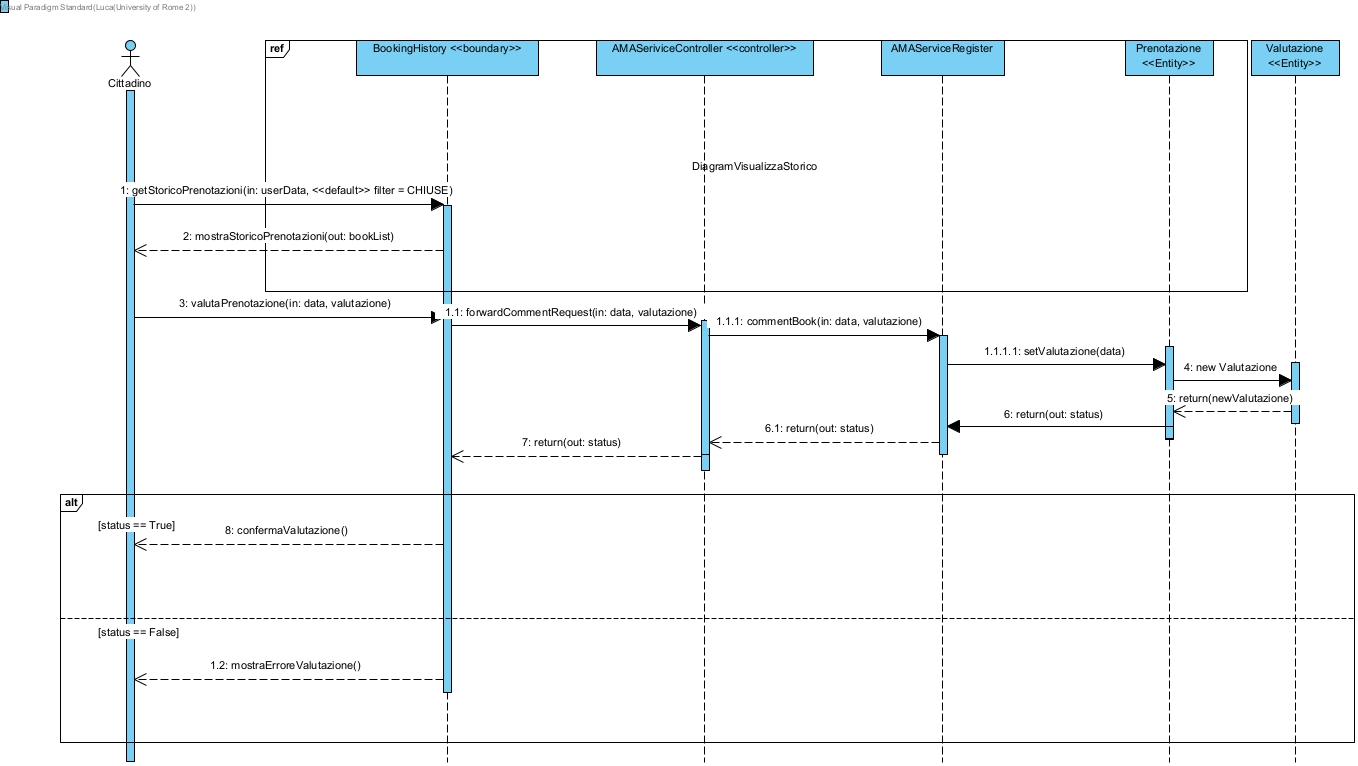
\includegraphics[width=\textwidth,height=0.70\textheight,keepaspectratio]{figure/seq_DiagramValutarePrenotazione.jpg}
    \caption{Sequence Diagram --- Valutare il servizio}
\end{figure}

\subsubsection{Autista AMA}

\begin{figure}[H]
    \centering
    
\includegraphics[width=\textwidth,height=0.70\textheight,keepaspectratio]{figure/seq_Visualizzare_ritiri_assegnati.jpg}
    \caption{Sequence Diagram --- Visualizzare ritiri assegnati}
\end{figure}

\begin{figure}[H]
    \centering
    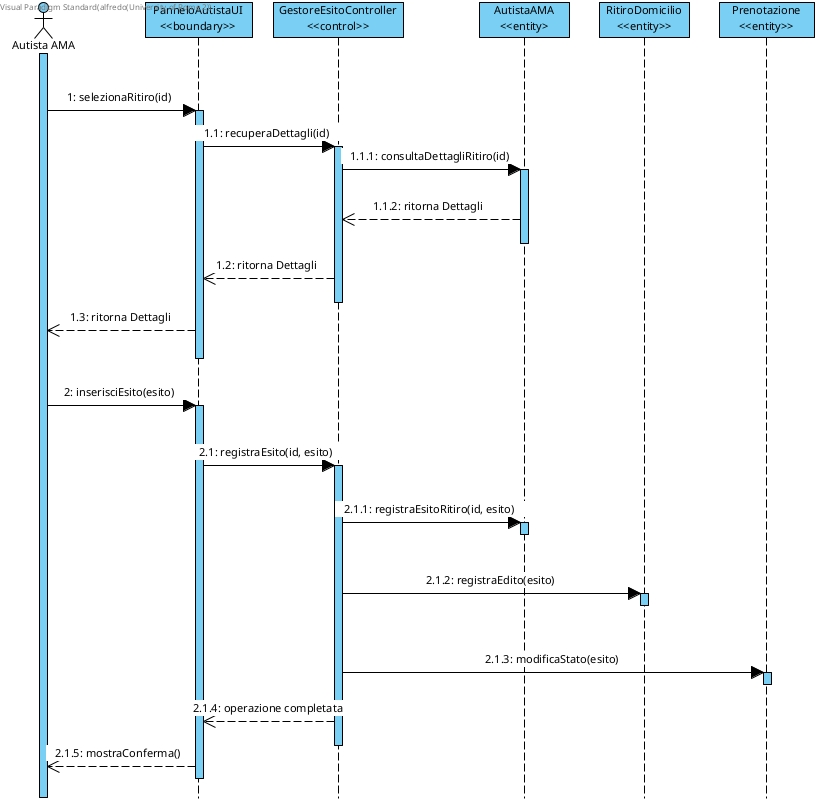
\includegraphics[width=\textwidth,height=0.70\textheight,keepaspectratio]{figure/seq_Registrare_esito_ritiro.jpg}
    \caption{Sequence Diagram --- Registrare esito del ritiro}
\end{figure}

\begin{figure}[H]
    \centering
    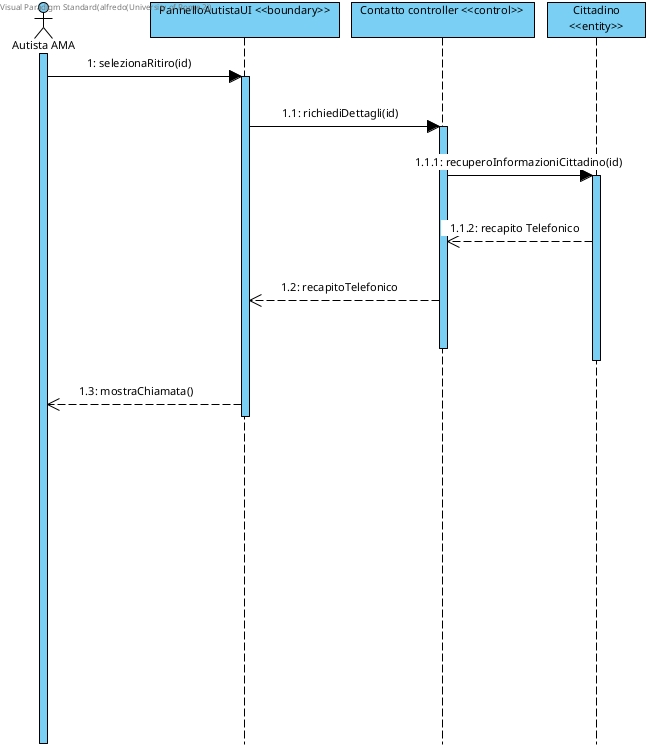
\includegraphics[width=\textwidth,height=0.70\textheight,keepaspectratio]{figure/seq_Chiamare_cittadino.jpg}
    \caption{Sequence Diagram --- Chiamare cittadino}
\end{figure}

\subsubsection{Operatore di Sede AMA}

\begin{figure}[H]
    \centering
    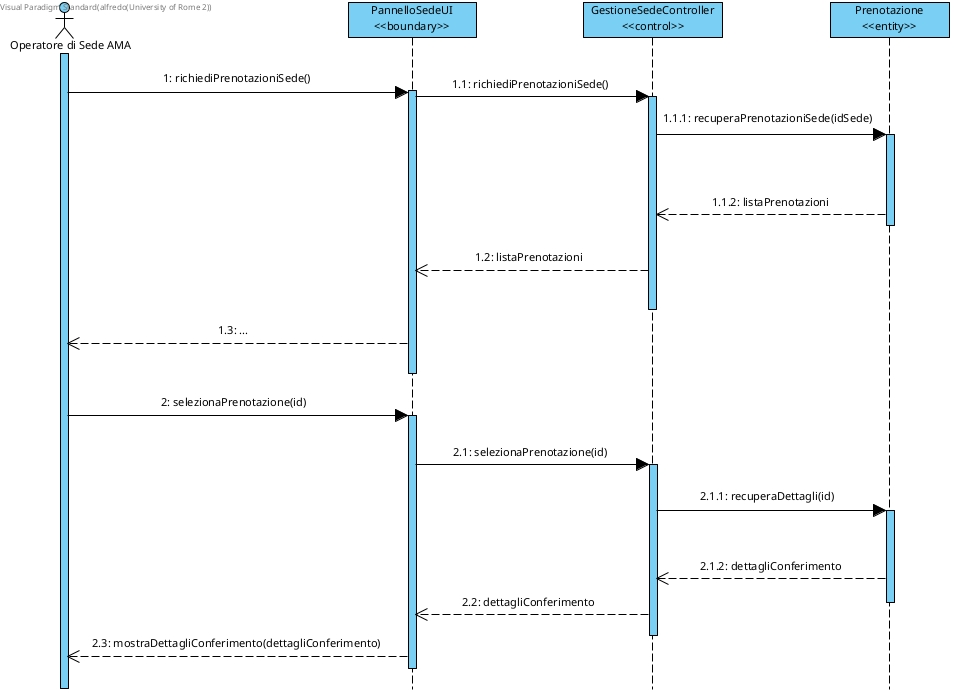
\includegraphics[width=\textwidth,height=0.70\textheight,keepaspectratio]{figure/seq_SequenceVisualizzarePrenotazioniSede.jpg}
    \caption{Sequence Diagram --- Visualizzare prenotazioni della sede}
\end{figure}

\begin{figure}[H]
    \centering
    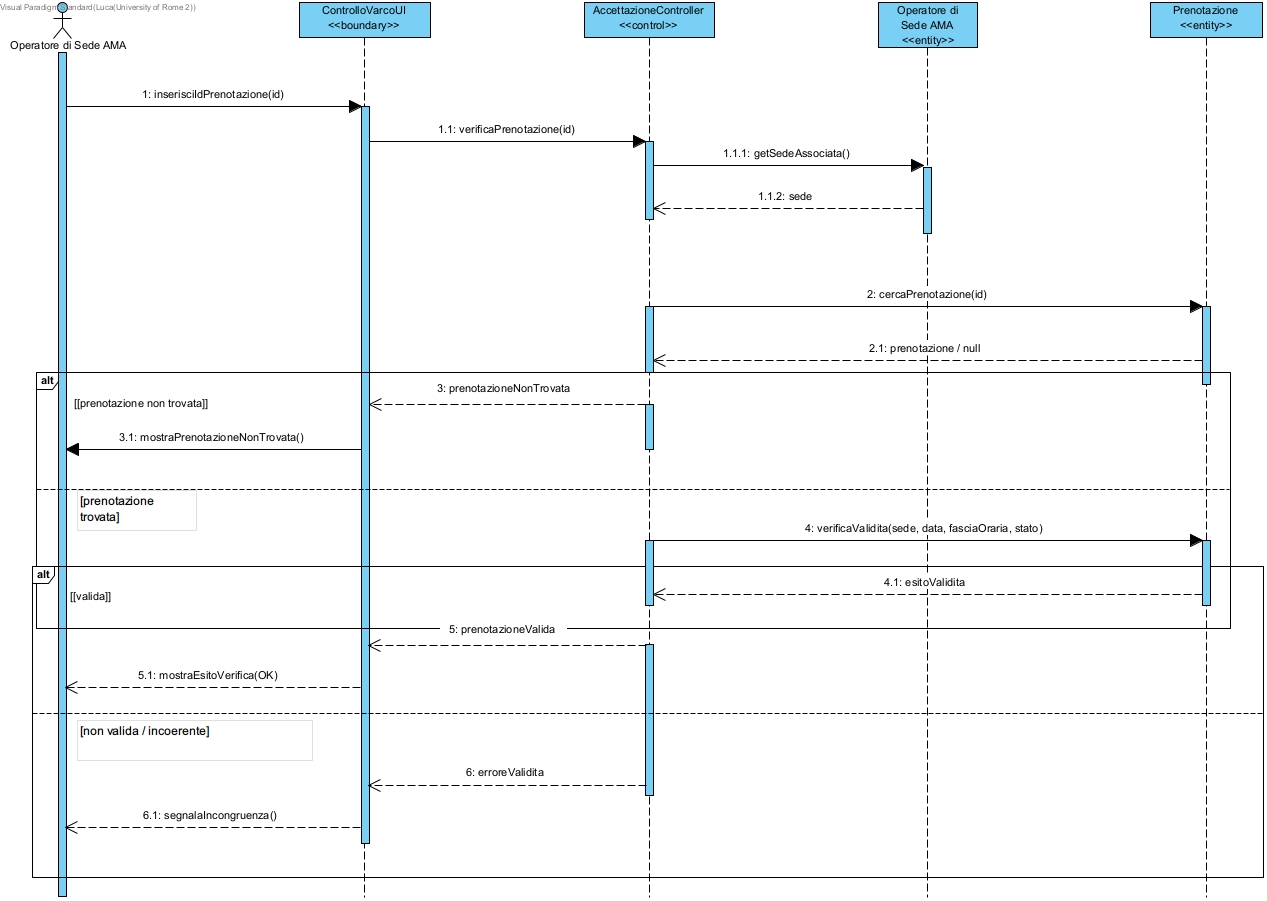
\includegraphics[width=\textwidth,height=0.70\textheight,keepaspectratio]{figure/seq_SequenceVerificarePrenotazioneCittadino.jpg}
    \caption{Sequence Diagram --- Verificare prenotazione del cittadino}
\end{figure}

\begin{figure}[H]
    \centering
    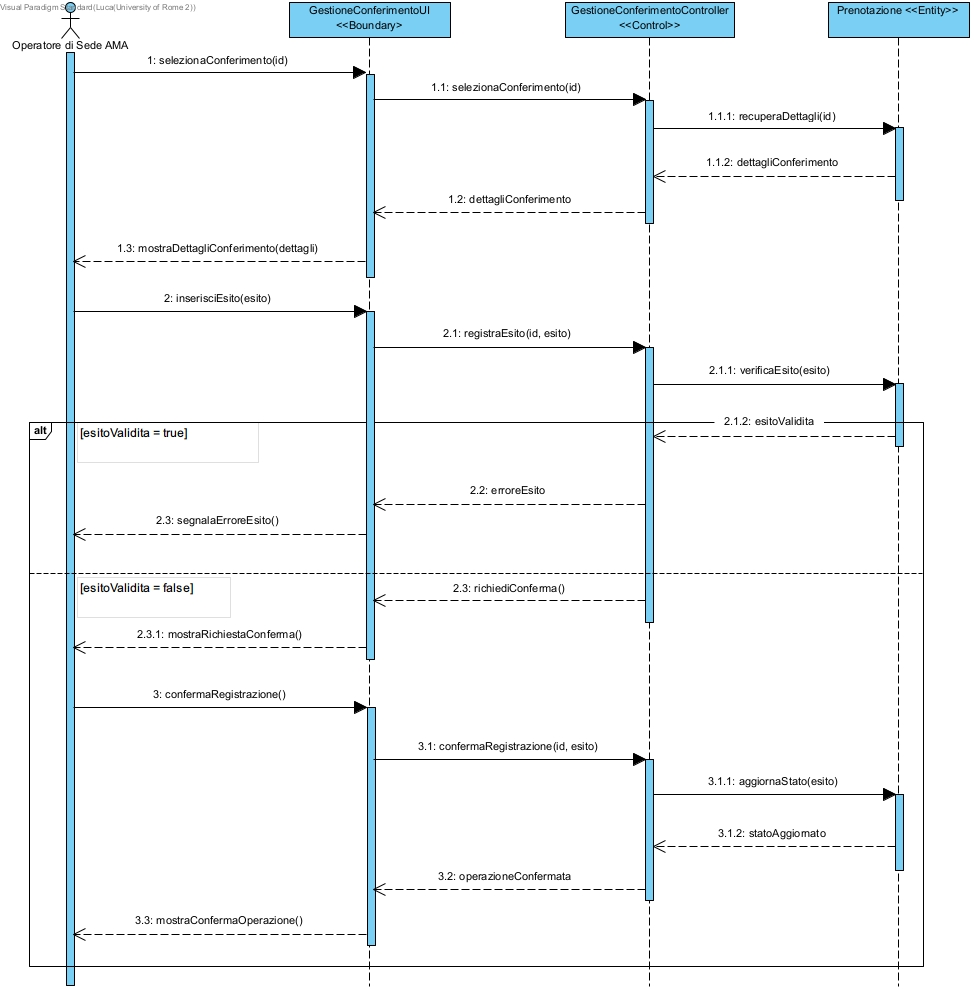
\includegraphics[width=\textwidth,height=0.70\textheight,keepaspectratio]{figure/seq_SequenceRegistrareEsitoConferimento.jpg}
    \caption{Sequence Diagram --- Registrare esito del conferimento}
\end{figure}

\subsubsection{Amministratore di Sede AMA}

\begin{figure}[H]
    \centering
    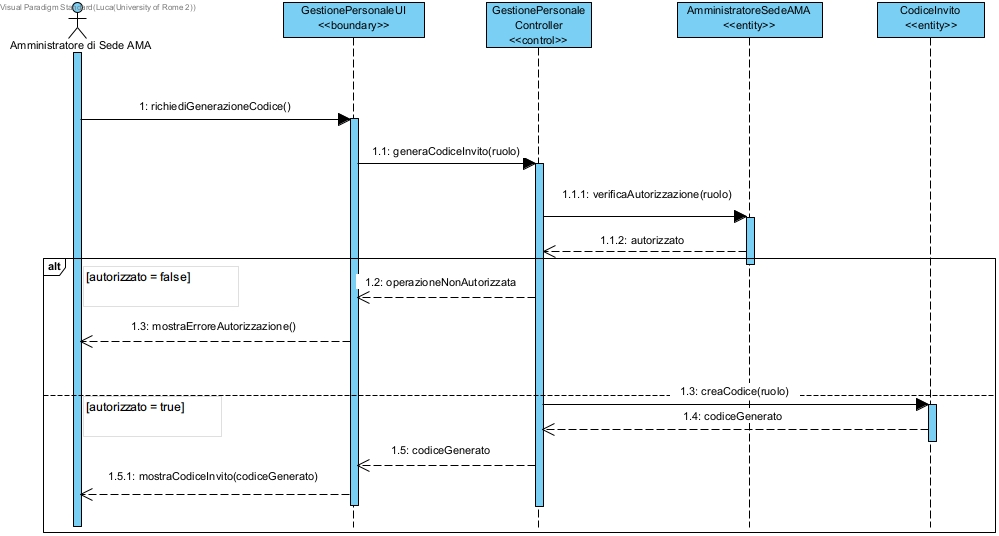
\includegraphics[width=\textwidth,height=0.70\textheight,keepaspectratio]{figure/seq_SequenceGenerareCodiceInvitoPersonale.jpg}
    \caption{Sequence Diagram --- Generare codice invito}
\end{figure}

\begin{figure}[H]
    \centering
    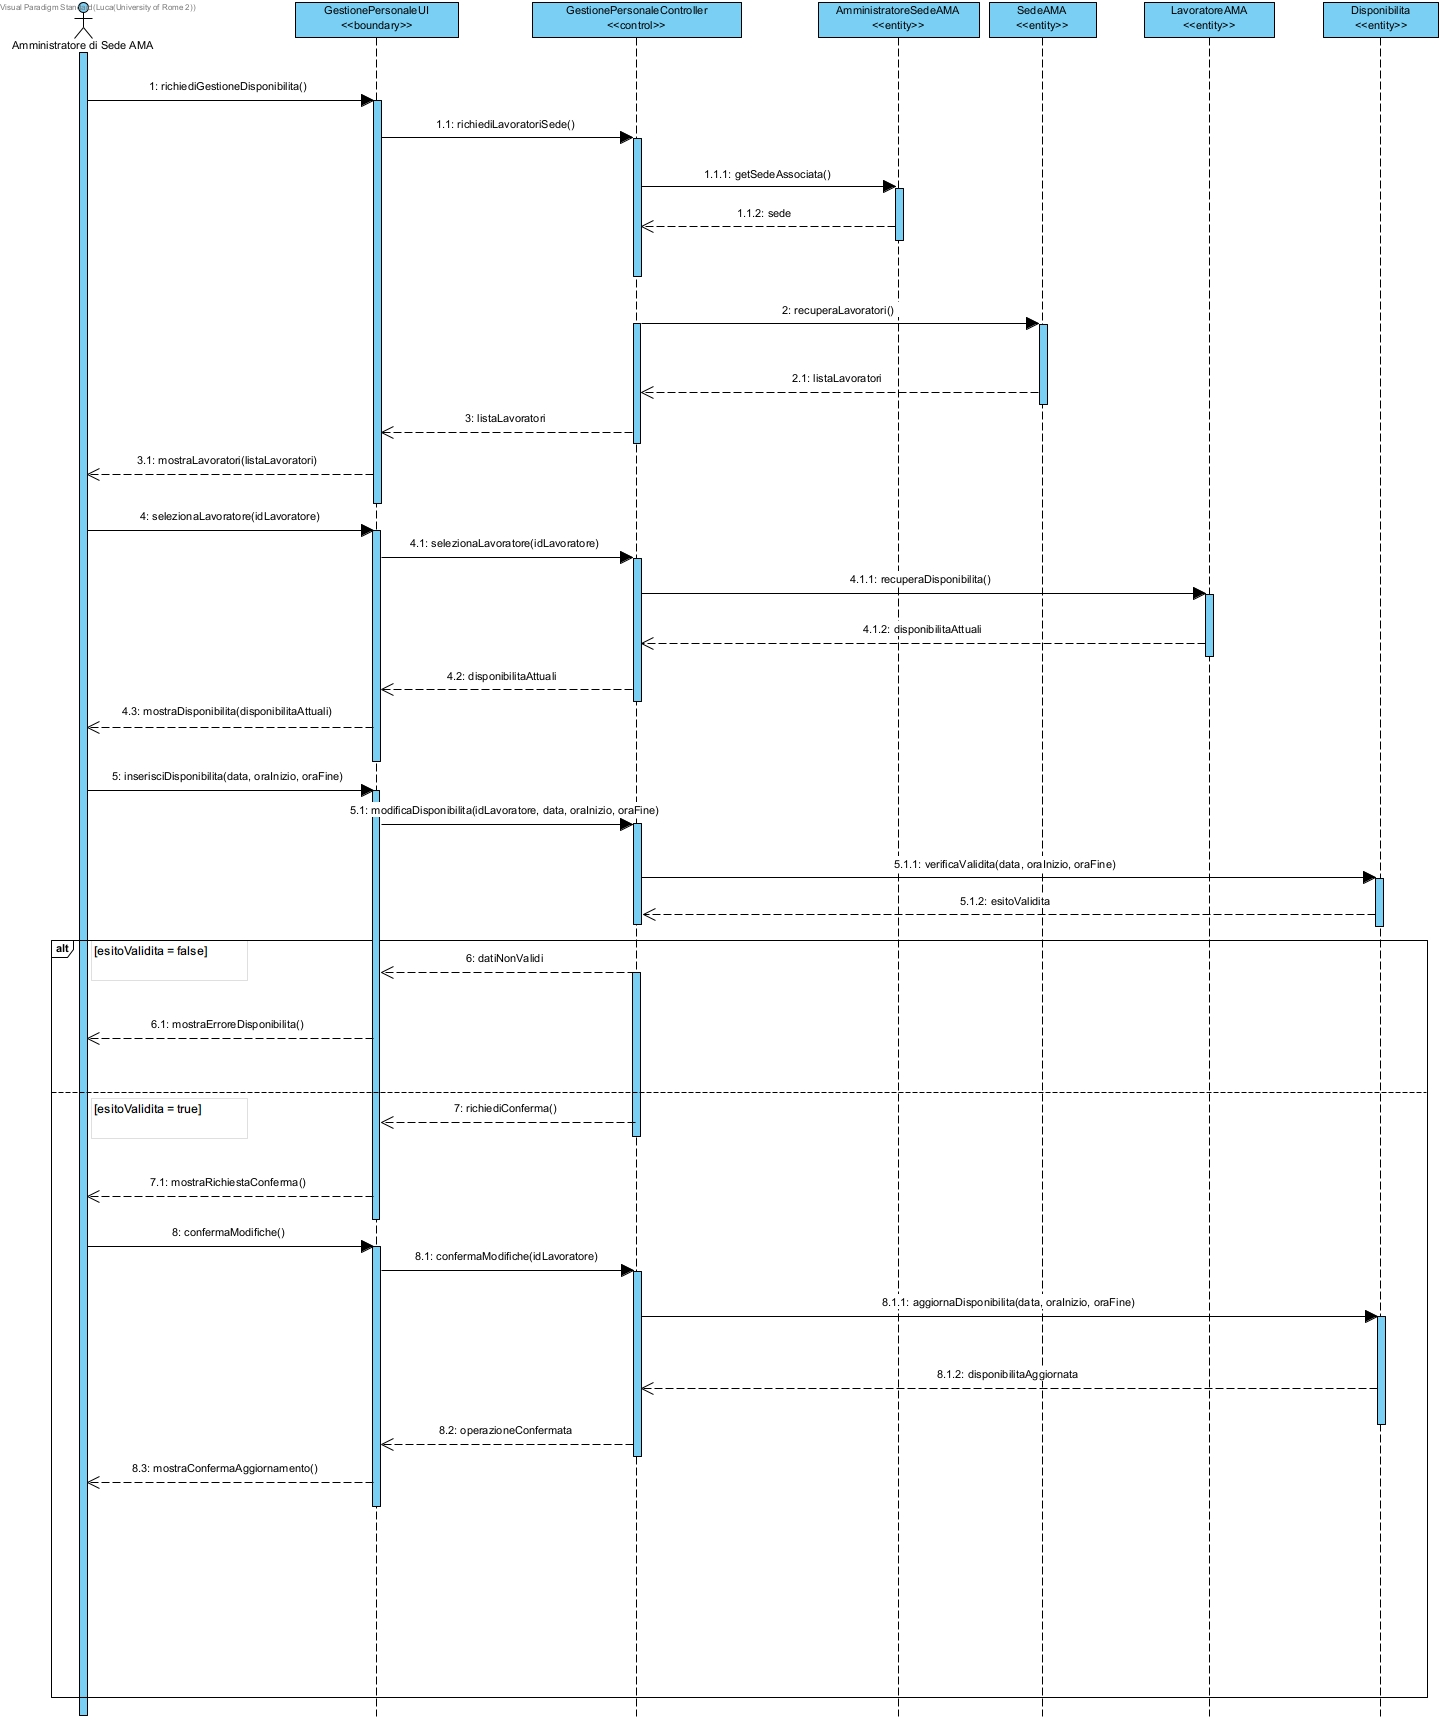
\includegraphics[width=\textwidth,height=0.70\textheight,keepaspectratio]{figure/seq_SequenceGestireDisponibilitaLavoratori.jpg}
    \caption{Sequence Diagram --- Gestire disponibilità dei lavoratori}
\end{figure}

\begin{figure}[H]
    \centering
    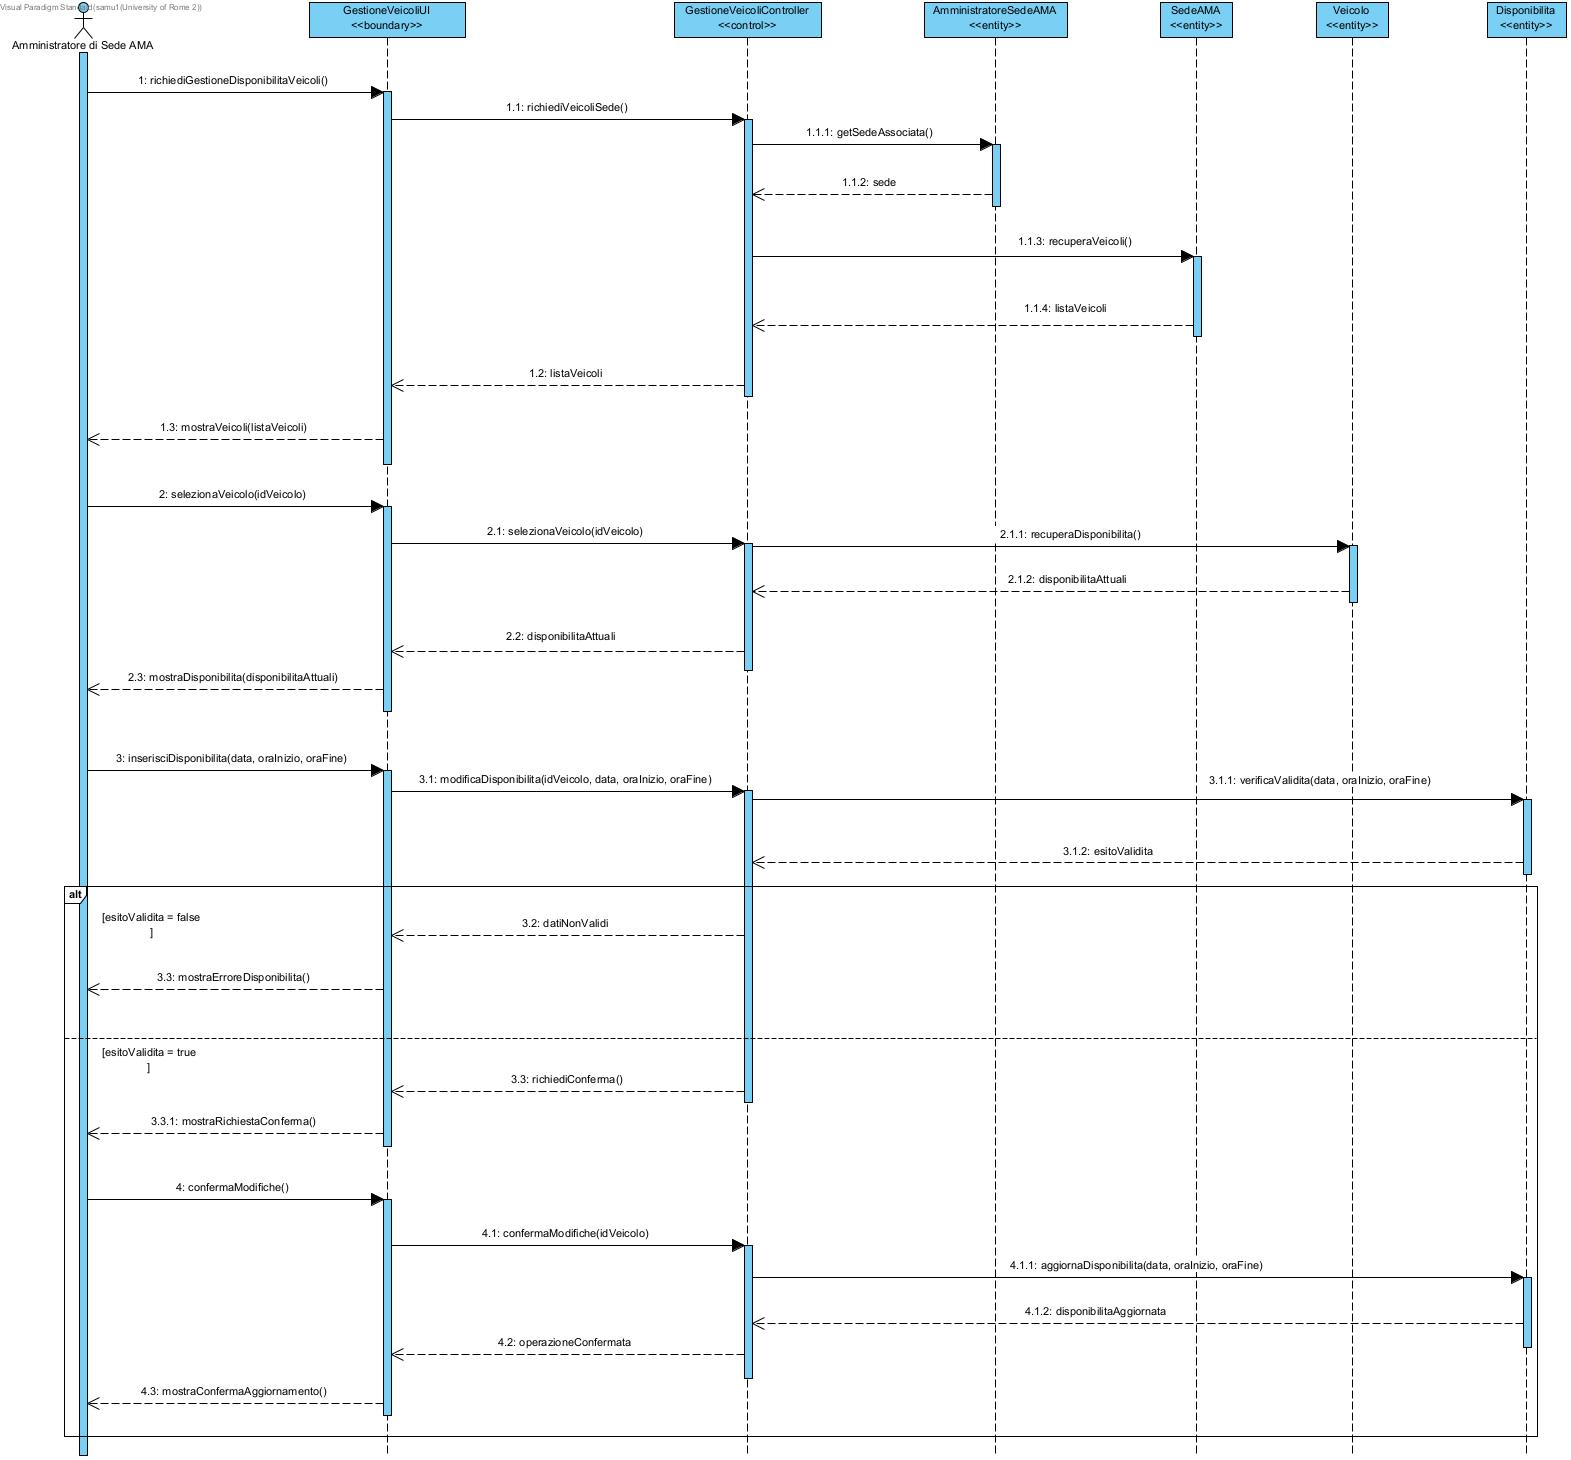
\includegraphics[width=\textwidth,height=0.70\textheight,keepaspectratio]{figure/seq_SequenceGestireDisponibilitaVeicoli.jpg}
    \caption{Sequence Diagram --- Gestire disponibilità dei veicoli}
\end{figure}

\begin{figure}[H]
    \centering
    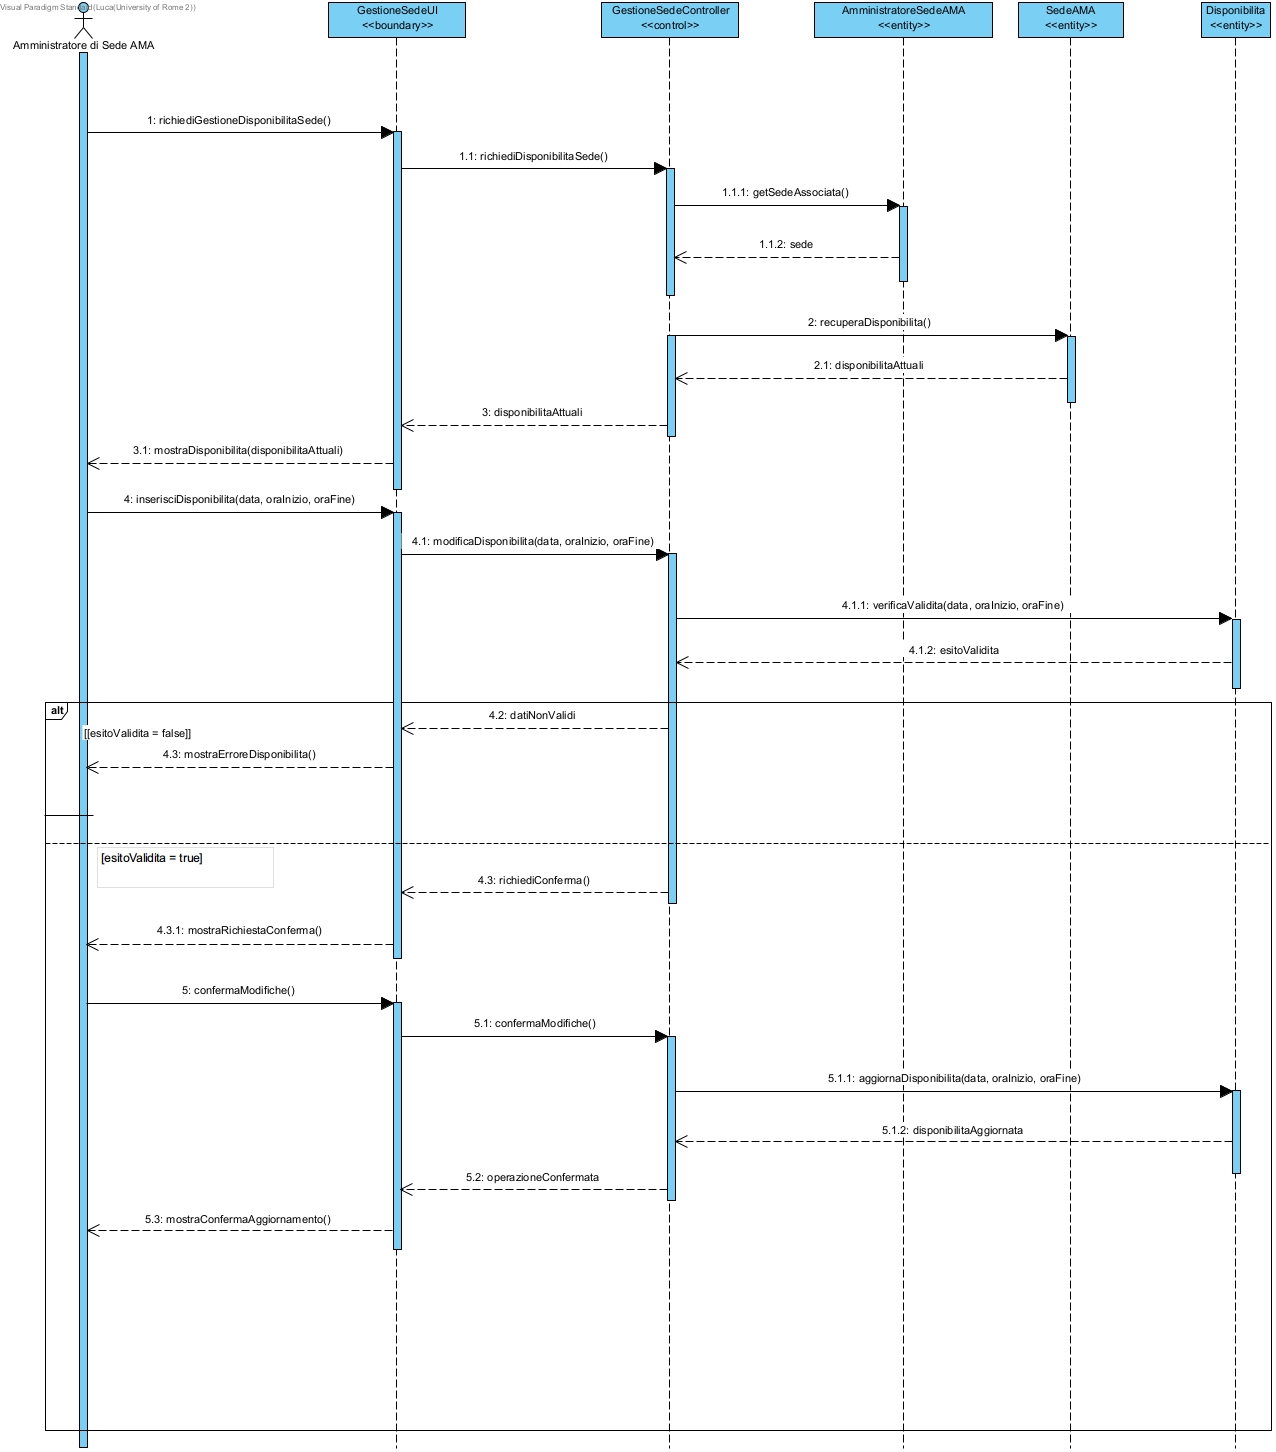
\includegraphics[width=\textwidth,height=0.70\textheight,keepaspectratio]{figure/seq_SequenceGestireDisponibilitaSede.jpg}
    \caption{Sequence Diagram --- Gestire disponibilità della sede e fasce orarie}
\end{figure}

\begin{figure}[H]
    \centering
    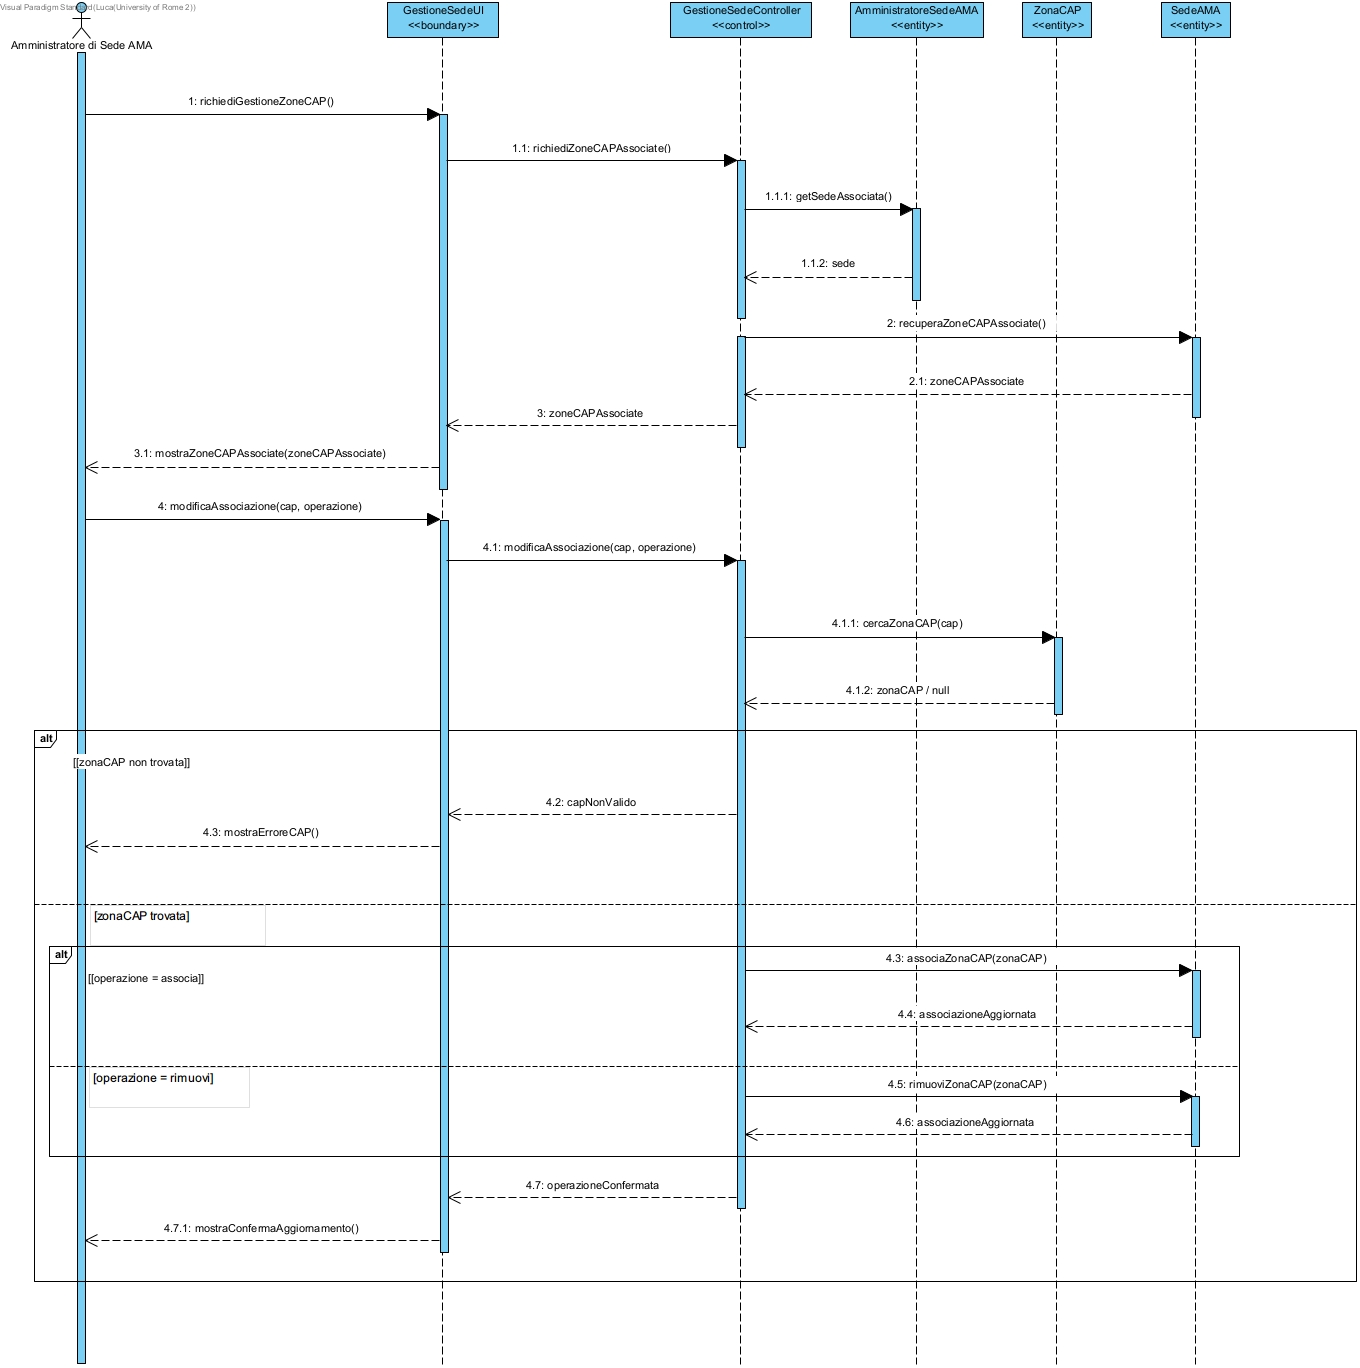
\includegraphics[width=\textwidth,height=0.70\textheight,keepaspectratio]{figure/seq_SequenceGestireAssociazioniSedeZoneCAP.jpg}
    \caption{Sequence Diagram --- Gestire associazioni tra sede e zone/CAP}
\end{figure}

\begin{figure}[H]
    \centering
    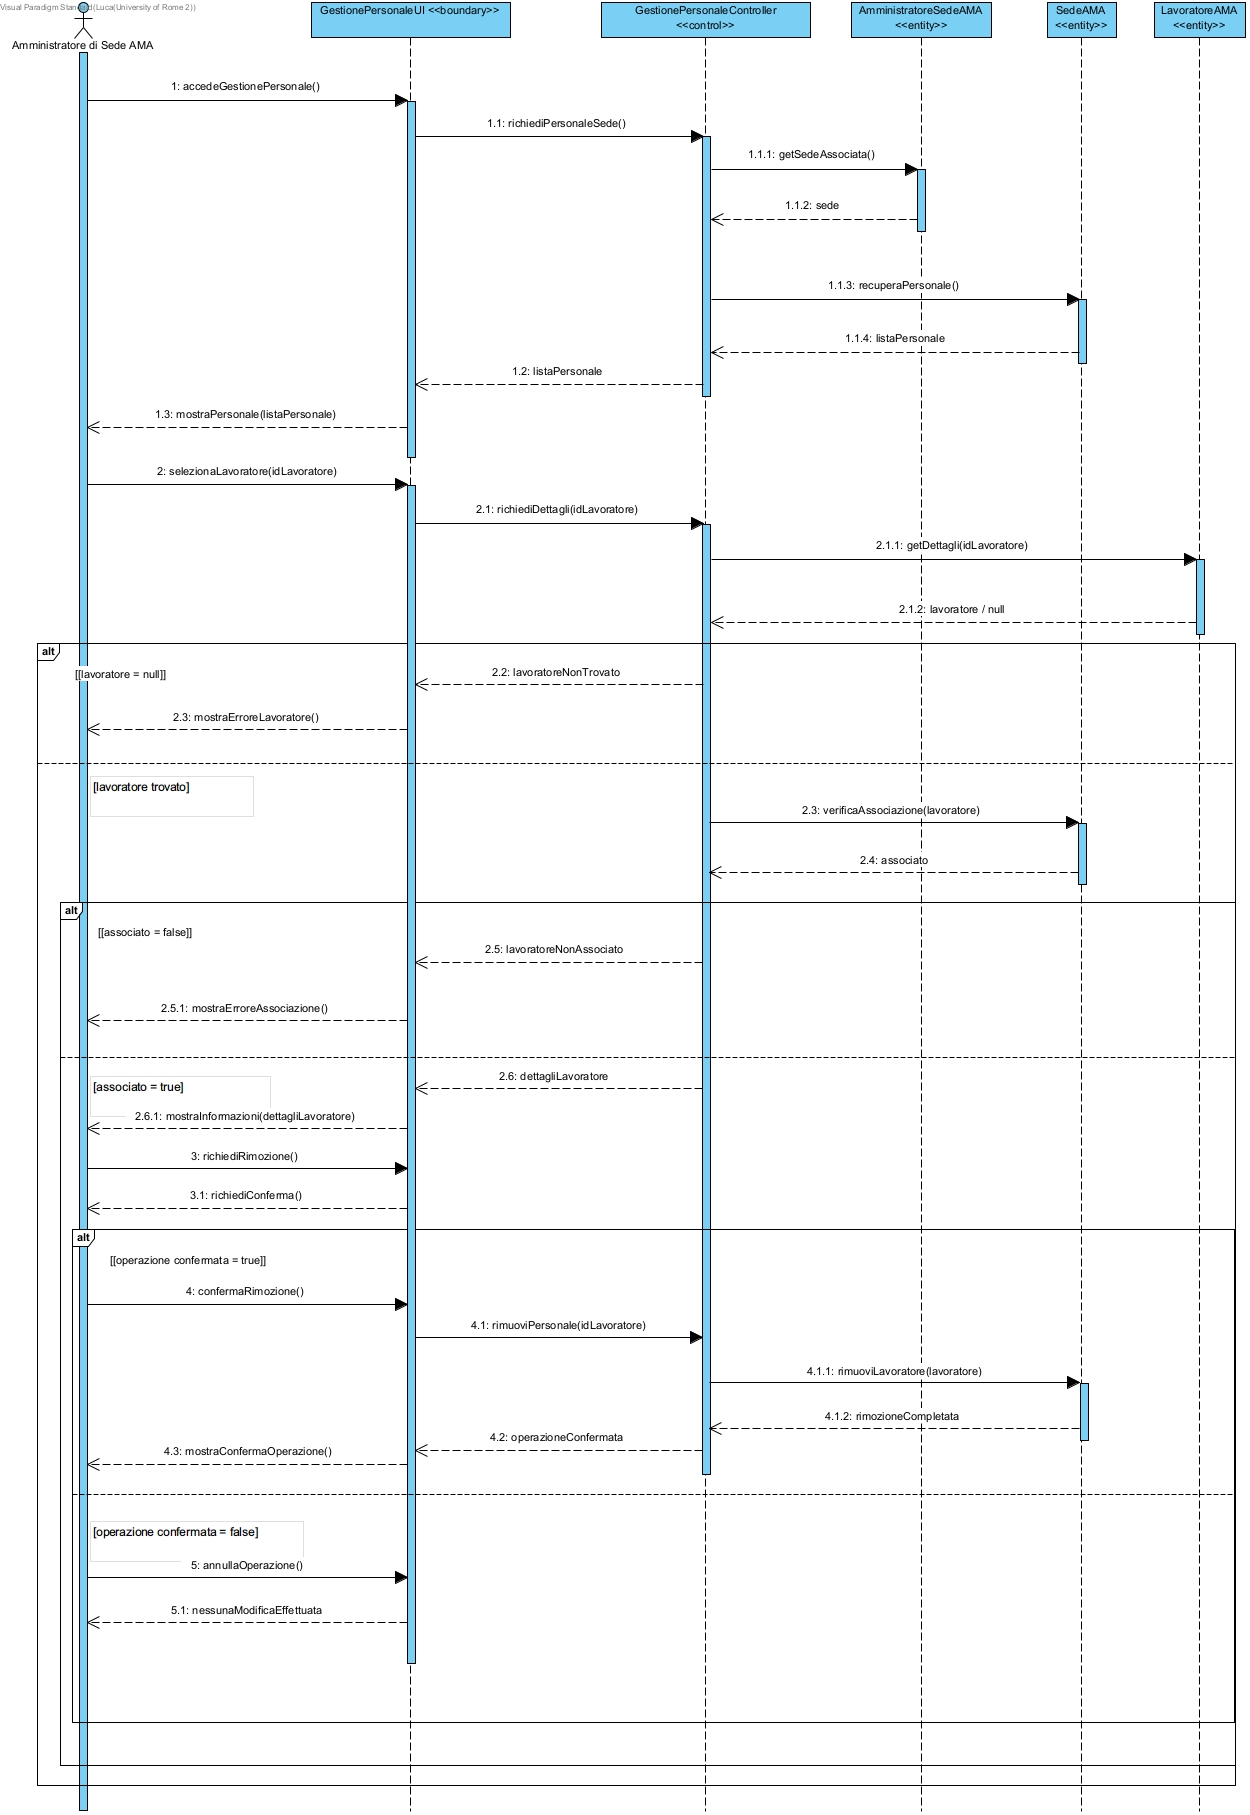
\includegraphics[width=\textwidth,height=0.70\textheight,keepaspectratio]{figure/seq_SequenceRimuoverePersonaleAMA.jpg}
    \caption{Sequence Diagram --- Rimuovere personale}
\end{figure}

\subsubsection{Amministratore Generale AMA}

\begin{figure}[H]
    \centering
    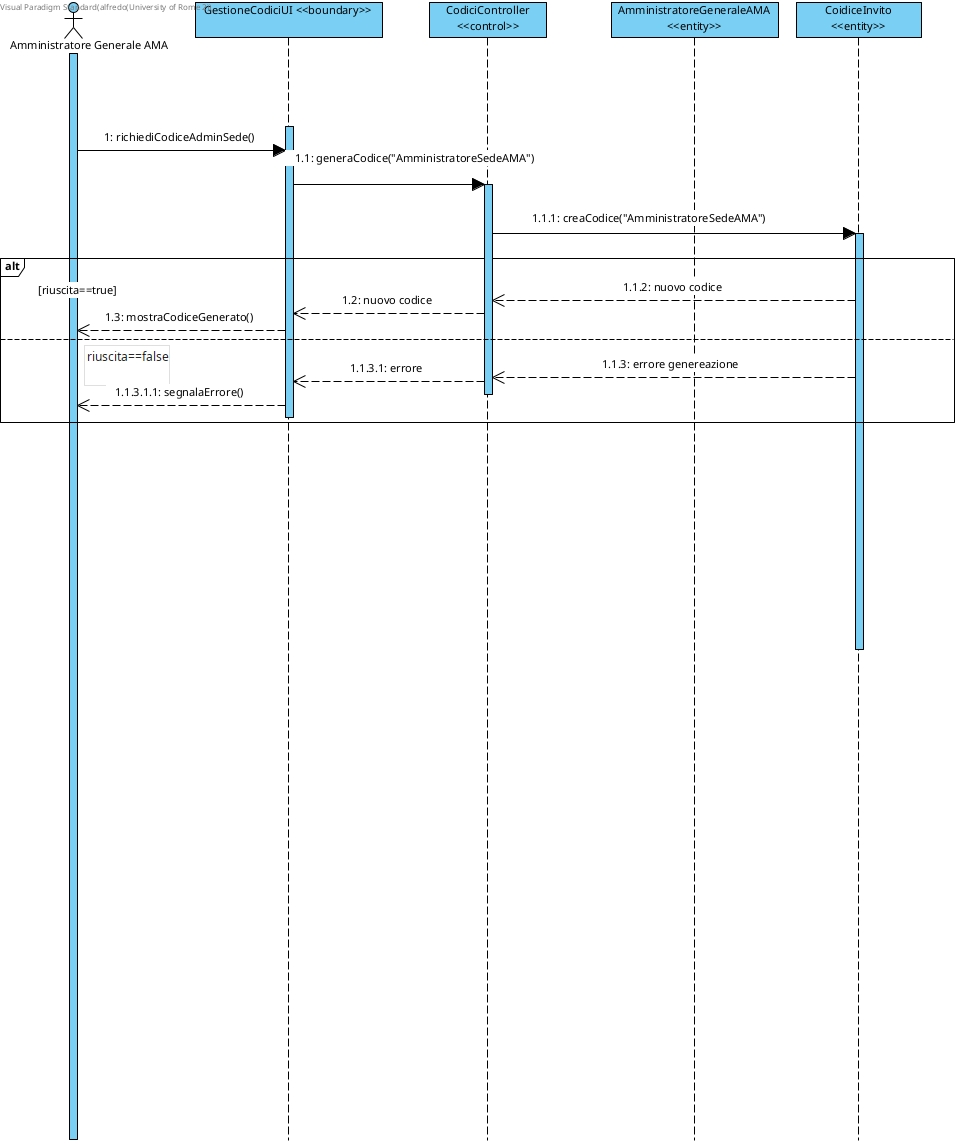
\includegraphics[width=\textwidth,height=0.70\textheight,keepaspectratio]{figure/seq_AmministratoreGeneraleGeneraCodici.jpg}
    \caption{Sequence Diagram --- Generare codice amministratore di sede}
\end{figure}

\begin{figure}[H]
    \centering
    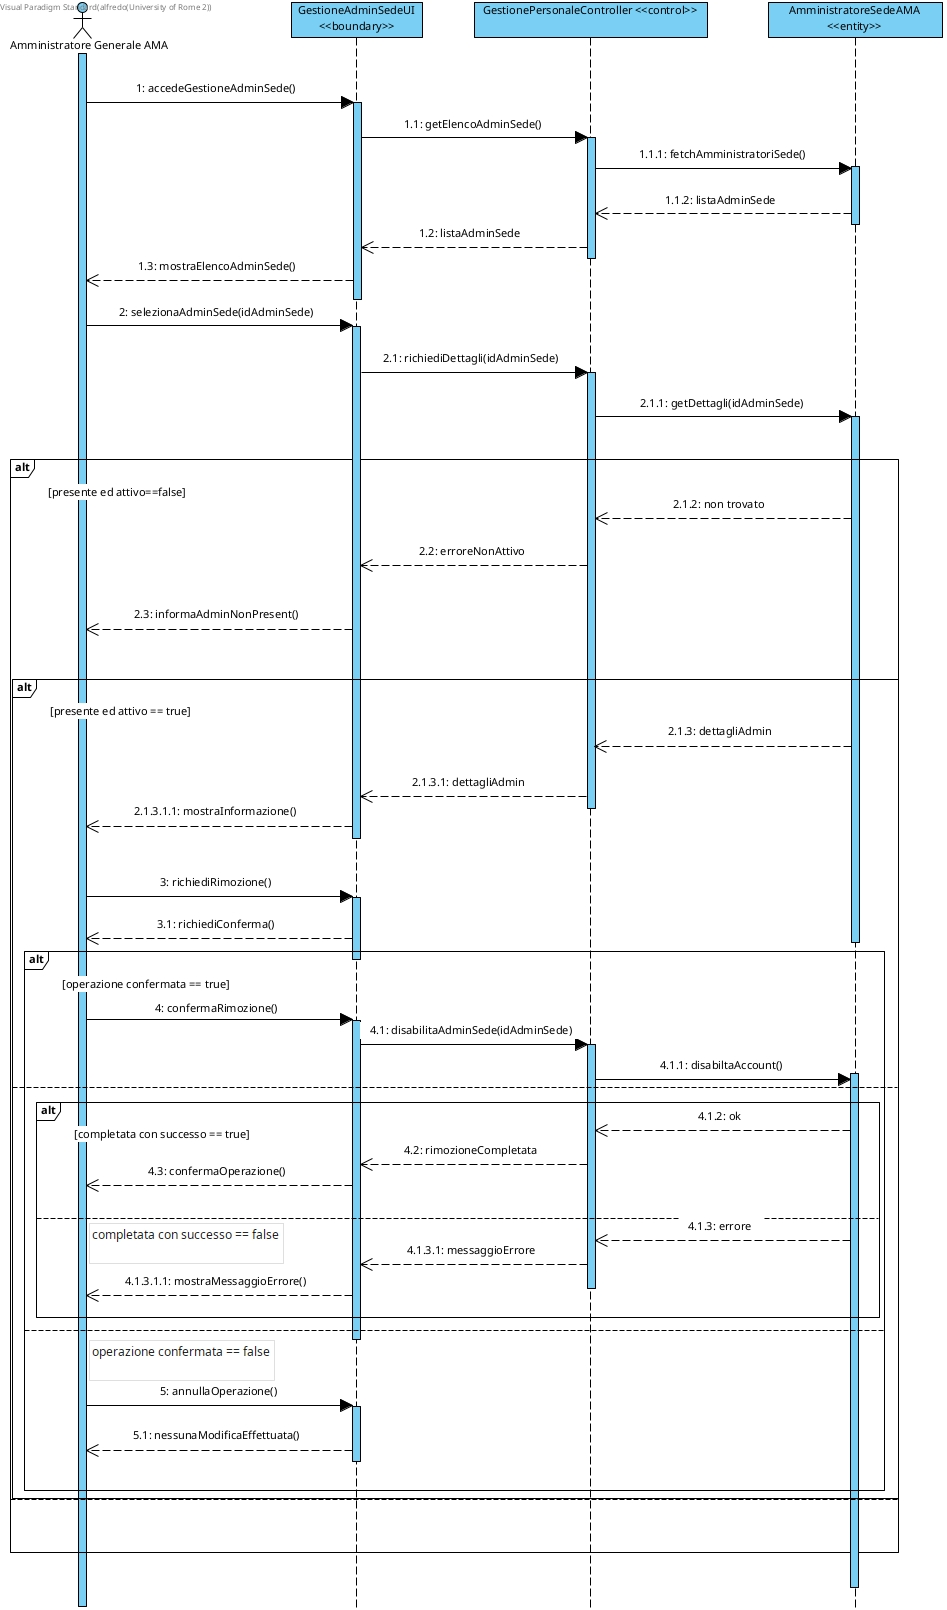
\includegraphics[width=\textwidth,height=0.70\textheight,keepaspectratio]{figure/seq_RimuovereAmministratoreDiSedeAMA.jpg}
    \caption{Sequence Diagram --- Rimuovere amministratore di sede AMA}
\end{figure}

% =========================================================================
% 5.3 CLASS DIAGRAMS
% =========================================================================
\subsection{Class Diagrams}
I Class Diagram rappresentano la struttura statica delle entità, le classi di controllo e interfaccia, gli attributi, i metodi e le relazioni (associazioni, aggregazioni, composizioni ed ereditarietà).

\subsubsection{Class Diagram Unrefined (Modello Concettuale di Dominio)}
Il modello \textit{Unrefined} illustra le entità concettuali e le loro relazioni primarie derivanti direttamente dall'analisi del dominio applicativo e dal glossario.

\begin{figure}[H]
    \centering
    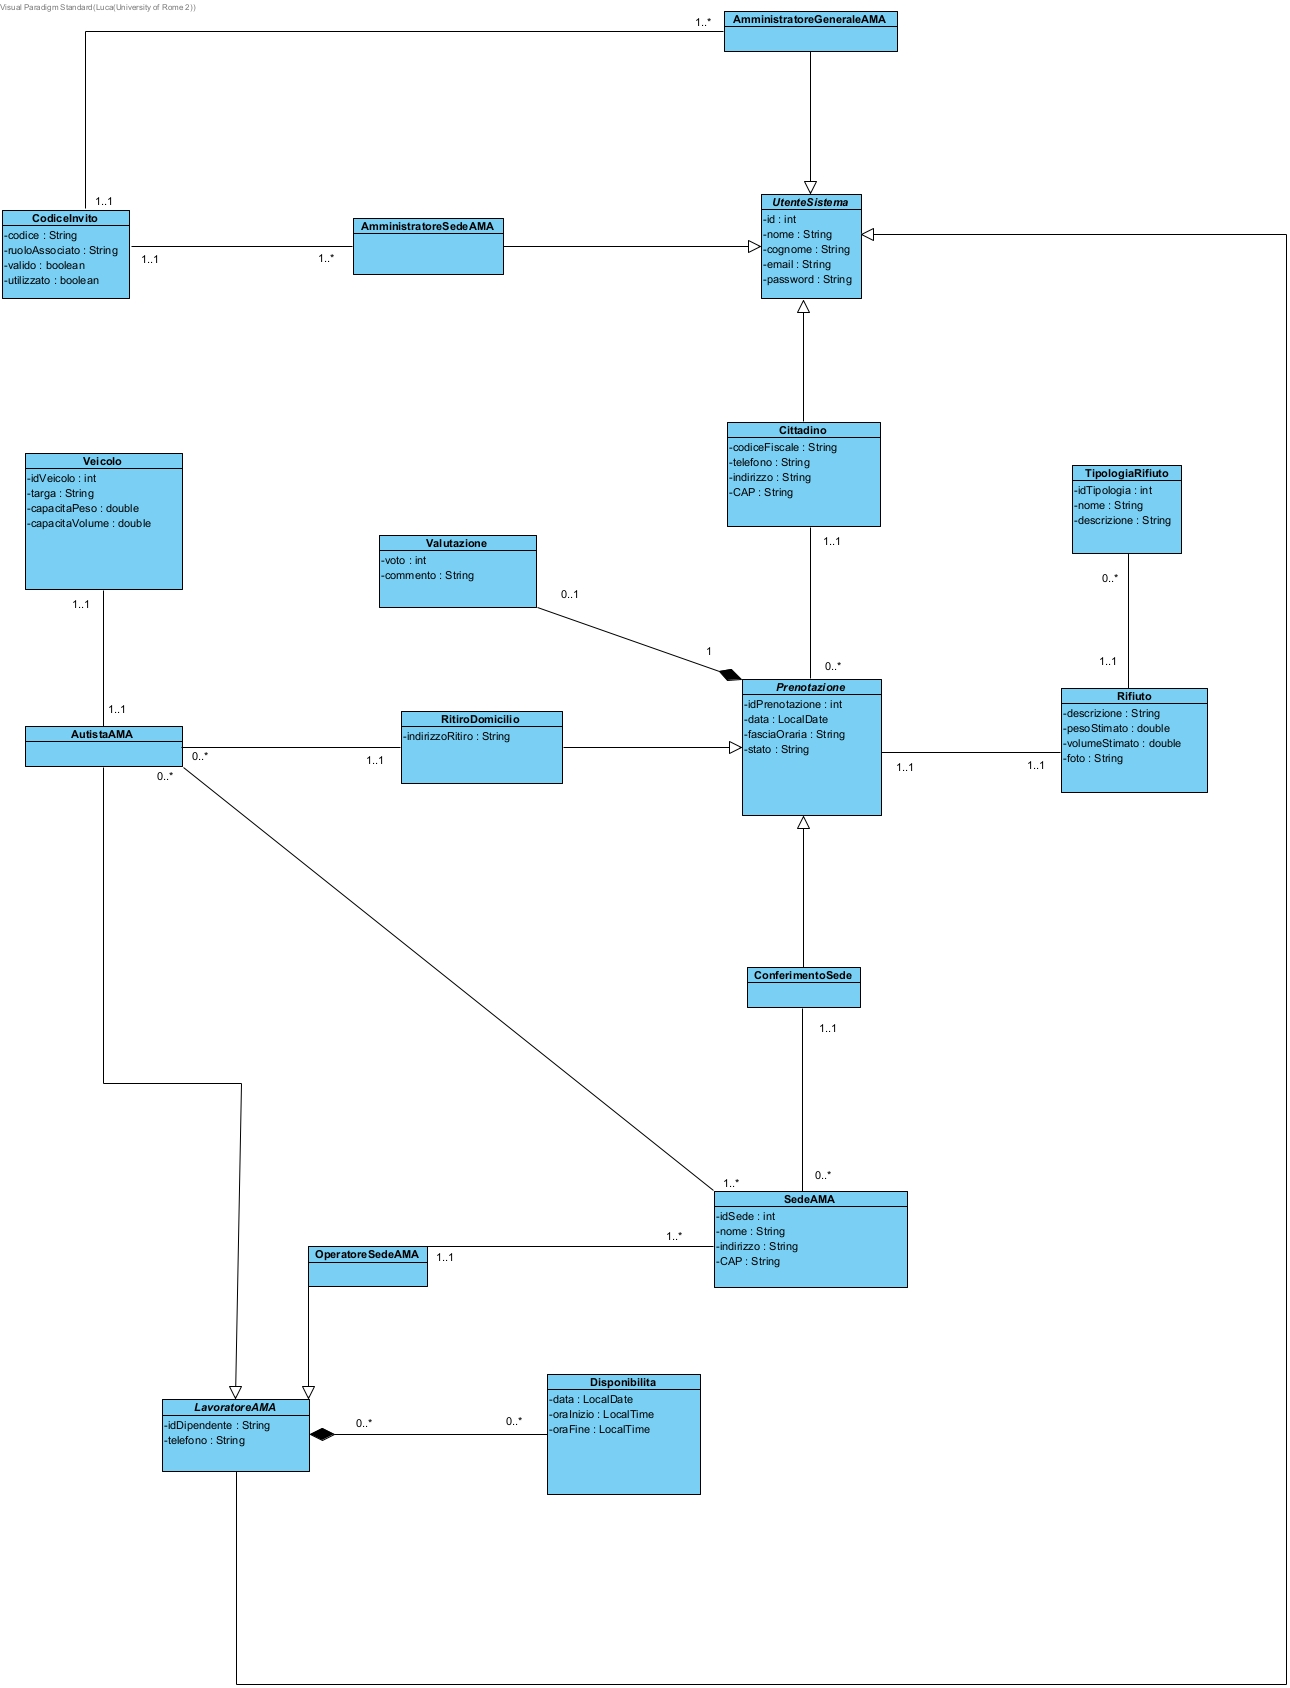
\includegraphics[width=\textwidth,height=0.80\textheight,keepaspectratio]{figure/class_CLASS_DIAGRAM_unrefined.jpg}
    \caption{Class Diagram --- Versione Unrefined (Modello di Dominio)}
    \label{fig:class_unrefined}
\end{figure}

\subsubsection{Class Diagram Refined (Modello di Progettazione Dettagliato)}
Il modello \textit{Refined} integra e consolida l'architettura completa a oggetti del sistema \textbf{MyAma}, strutturando le classi secondo il pattern architetturale BCE (\textit{Boundary, Control, Entity}). In esso vengono specificati esaustivamente tutti gli attributi con la relativa visibilità e tipo, i metodi operativi derivati dai Sequence Diagram, nonché le relazioni complete con navigabilità e molteplicità.

\begin{figure}[H]
    \centering
    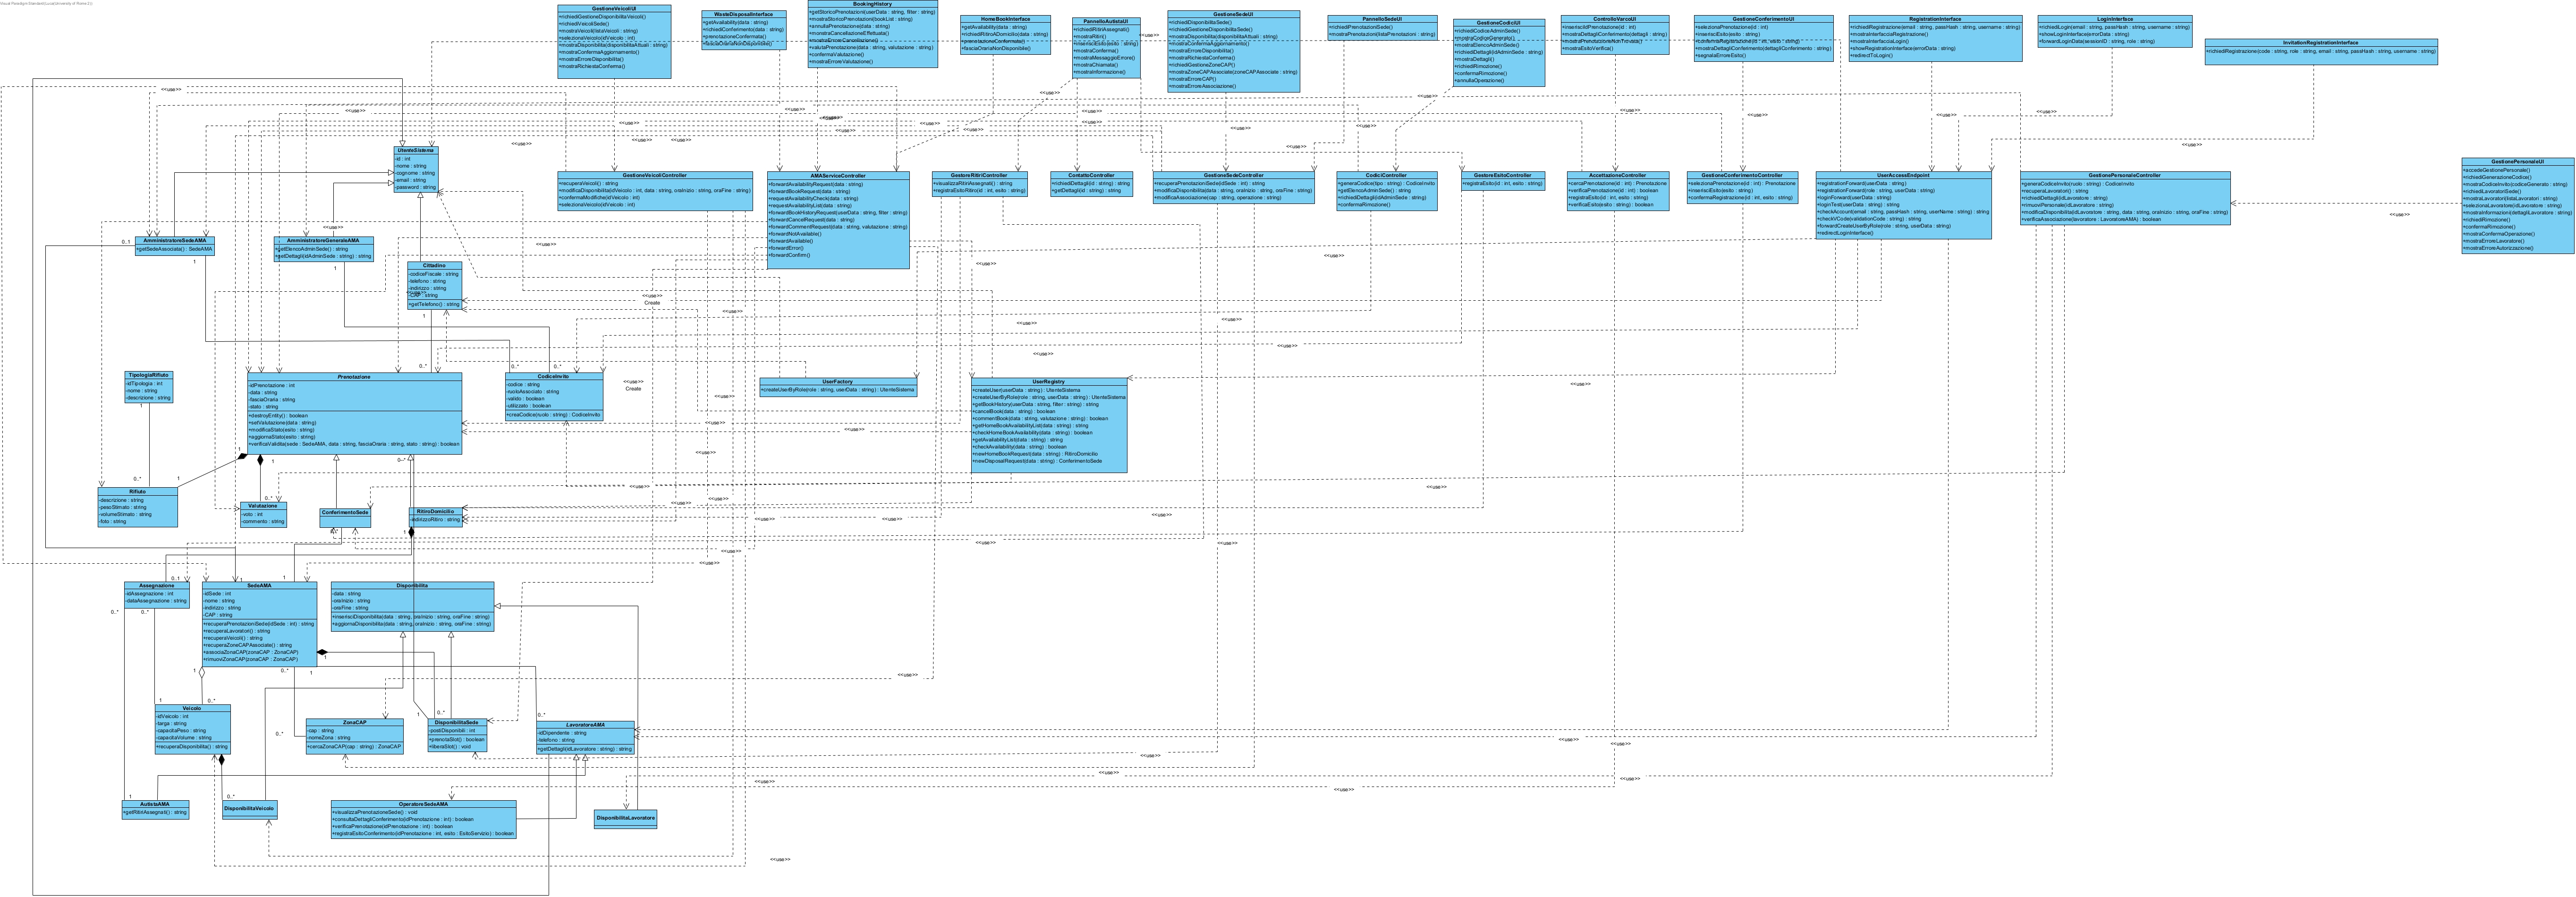
\includegraphics[width=\textwidth,height=0.85\textheight,keepaspectratio]{figure/class_CLASS_DIAGRAM_refined.jpg}
    \caption{Class Diagram --- Versione Refined (BCE e Struttura Consolidata)}
    \label{fig:class_refined}
\end{figure}
